\documentclass[english]{tktltiki}
%\documentclass[a4paper]{article}
%\usepackage[utf8]{inputenc}
\usepackage[pdftex]{graphicx}
%\usepackage{subfigure}
\usepackage{subcaption}
\usepackage{alltt}
\usepackage{gensymb} % for \textdegree
\usepackage{amsmath}
\usepackage{amssymb}
% for algorithmic typesetting
\usepackage{algpseudocode}
\usepackage{algorithm}
% break on long hyphens to prevent overstepping bounds
%\usepackage[hyphenbreaks]{breakurl} 
%\usepackage[hyphens]{url}
% to force 1-in margins
%\usepackage[margin=1in]{geometry}
\usepackage{enumitem} % for separation specifications

\usepackage{tikz}
\usetikzlibrary{matrix,positioning,arrows,decorations.pathmorphing,decorations.pathreplacing}

% argmin and argmax for typesetting
\DeclareMathOperator*{\argmin}{argmin}
\DeclareMathOperator*{\argmax}{argmax}

% expectation standardization
\newcommand{\Expectation}{\mathbb{E}}

% allow \paragraph as if it were \subsubsubsection
% also extend to \subparagraph by using 5
\setcounter{tocdepth}{5}
\setcounter{secnumdepth}{5}

% define \States, \Actions, \Policies for later
\newcommand{\Reals}{\mathcal{R}}
\newcommand{\States}{\mathcal{S}}
\newcommand{\Actions}{\mathcal{A}}
\newcommand{\Policies}{\mathcal{P}}
\newcommand{\policy}{\pi}

% define \Iarrow and \Earrow for value iteration math formula
\newcommand{\Iarrow}{\xrightarrow{I}}
\newcommand{\Earrow}{\xrightarrow{E}}

% p-vector simplicity
% # BSD sed b/c mac
% sed -i '' -e 's#\$p\$#\\pvec\\#g'
% similar for S & w
\newcommand{\pvecm}{\overline{p}}
\newcommand{\pvec}{$\pvecm$}
\newcommand{\Smatm}{\mathbf{S}}
\newcommand{\Smat}{$\Smatm$}
\newcommand{\wvecm}{\overline{w}}
\newcommand{\wvec}{$\wvecm$}

% Allow for line-breaking of true-type fonts on underscores
%	see: https://tex.stackexchange.com/questions/315369/how-to-deal-with-bad-line-wrapping-of-texttt
\newcommand*\ttwrap[1]{\texttt{\expandafter\dottvar\detokenize{#1}\relax}}
\newcommand*\dottvar[1]{\ifx\relax#1\else
  \expandafter\ifx\string_#1\string_\allowbreak\else#1\fi
  \expandafter\dottvar\fi}

% define strategy names to avoid having to type \texttt{a\_b\_c} so much
\newcommand{\handmaxmin}{\ttwrap{hand_max_min}}
\newcommand{\handmaxavg}{\ttwrap{hand_max_avg}}
\newcommand{\handmaxmed}{\ttwrap{hand_max_med}}
\newcommand{\handmaxposs}{\ttwrap{hand_max_poss}}
\newcommand{\cribminavg}{\ttwrap{crib_min_avg}}
\newcommand{\peggingmaxavggained}{\ttwrap{pegging_max_avg_gained}}
\newcommand{\peggingmaxmedgained}{\ttwrap{pegging_max_med_gained}}
\newcommand{\peggingminavggiven}{\ttwrap{pegging_min_avg_given}}

% learned --> learne'd
% really only allowed in poetry and literature,
% so will have to reset to just learned
\newcommand{\learned}{learned}

% card suits for easier text-mode use later
\newcommand{\hearts}{$\heartsuit$}
\newcommand{\clubs}{$\clubsuit$}
\newcommand{\diamonds}{$\diamondsuit$}
\newcommand{\spades}{$\spadesuit$}

%%% Source for figures for my safety
\newcommand*{\captionsource}[2]{%
	\caption[{#1}]{%
		#1%
%		\\\hspace{\linewidth}%
%		\textbf{Source:} #2%
	}%
}
%%%

\title{Policy Improvement in Cribbage} % through Reinforcement Learning}
\author{Sean R. Lang}
\date{\today}

\begin{document}
%\doublespacing
%\singlespacing
%\onehalfspacing

\maketitle

\numberofpagesinformation{\numberofpages\ pages + \numberofappendixpages\ appendices}
\classification{\protect{\ \\
		I.2 [ARTIFICIAL INTELLIGENCE],\\
		I.2.1 [Applications and Expert Systems],\\
		I.2.6 [Learning]\\
		%A.1 [Introductory and Survey],\\
		%H.5.1 [Artificial, augmented, and virtual realities],\\
		%I.3.7 [Virtual Reality]
	}
}

\keywords{machine learning, reinforcement learning, cribbage}

\begin{abstract}

%%%
% Abstract of the thesis.
% One or two sentences on each of the topics covered in the thesis
%%%

%%%
Cribbage is a card game involving multiple methods of scoring
which each receive varying emphasis
over the course of a typical game.
%
Reinforcement learning is a machine learning strategy in which an agent learns
to accomplish a task via direct experience
by collecting rewards based on performance.
%
In this thesis,
reinforcement learning is applied to the game of cribbage,
improving an agent's policy of combining multiple basic strategies,
according to the needs of dynamic state of the game.
% TODO: ^^^ still need to rewrite this craptacular sentence
%
From inspection,
a reasonable policy is learned by the agent over the course of a million games,
but an increase in performance was not demonstrated.
%%%

\end{abstract}


\section*{Acknowledgments}

%%%
% Thanks for each person involved in this
%	Parents (duh)
%	Dr. Roos (mentor)
%	Chelsea (editing)
%	University (opportunity)
%%%

%%%
I would like to thank my parents, Kevin and Debra Lang,
for supporting me
throughout the years and especially in the decision to pursue a master's degree
in the distant land of Finland.
%
I would also like to thank Drs. Teemu Roos
and Jukka Kohonen
for %his
their mentorship throughout the
process of developing and writing this thesis.
%
Thanks also to Chelsea Dunham for her help in editing and proofreading
this paper,
without whose help writing quality would surely have suffered.
%
Additionally,
a courteous thank you to Matt Jennings at
\ttwrap{dailycribbagehand.org} for providing a data dump
which could be used to compare my model against decisions humans made
in a variety of situations.
% ^^^ TODO: ensure actually used
%
Finally, my gratitude is extended to the University of Helsinki for the
opportunity to pursue my studies here.
%%%

%%%
% According to
% <https://www.aje.com/en/arc/editing-tip-writing-acknowledgments/>,
% these are not to include parents,
% but should include other institutional help: Kale(?)
%%%

\newpage


\mytableofcontents

\section{Introduction}

%%%
I just want to see if unicode characters will appear.
Jag måste se om unicode-characterer funger.
minä haluan katsoa kirjain öööö.
%%%

%%%
Generic introductory stuff giving a sentence or probably a paragraph about
each of the sections covered.
%%%


%%%
% Introduction
%	Research objectives/questions
%	Structure of the thesis
%%%


%%%
% An introductory overview of the game of cribbage.
% Complete in its coverage so that someone can start playing, but won't know
%	the exact scoring at all given times.
%%%

\subsection{Cribbage}

%%%
Cribbage is a multi-phase card game, typically played between two opposing
players.
%
While variants exist for three or more players, this paper will focus on the
two-player variant.
%
The game presents an interesting research area because of its unique scoring
methodology:
each hand is counted in two slightly different ways within each round and the
first player to reach as score of 121 points or more is declared the winner.
%
Players will usually keep track of their points by \textit{pegging} them on a 
characteristic board.
%
Because of its atypical win condition, different strategies hold differing
levels of importance throughout the game.
%%%


\subsubsection*{Rules of the Game}

%%%
In order to be able to understand the crucial nature of the temporally dependent
strategies, the rules and flow of a game of cribbage must be fully understood.
%
%While a more complete set of scoring rules can be found in Appendix
%~\ref{app:scoring_rules} and a complete set of tournament rules can be found
%at \cite{ACC_rules},
While a complete set of tournament rules can be found at~\cite{ACC_rules}
or~\cite{ACC_rulebook},
what follows is an overview complete enough such that a novice player,
following the scoring rules found in Appendix~\ref{app:scoring_rules},
could play a complete game.
%%%

%%%
The zeroth step, taken once per game, is to determine which player will be the
dealer for the first round and who will be the pone.
%
%The player who is not the dealer is called the pone.
%
In order to determine these roles,
each player cuts the deck once to get a single card:
the player with the lower-valued card%
\footnote{Ace < 2 < 3 < 4 < 5 < 6 < 7 < 8 < 10 < Jack < Queen < King}
is the dealer;
the other player is called the pone.
%\footnote{
In the case of a tie, this step is repeated until two unique cards are
cut from the deck.
%}
%
From there, the usual round structure begins and proceeds in the following
steps:
%
\begin{enumerate}
%
\item Each player is dealt 6 cards.
%
\item Each player selects 4 cards to keep for their own hand and 2 cards to
	discard, or toss, into what is called the crib.
%
\item A random card is cut from the remaining cards of the deck and placed
	face-up on top of the deck.
	%
	If this cut card is a Jack of any suit,
	the dealer is awarded 2 points and pegs the points accordingly.
%
\item Starting with the pone, each player alternates playing a single card,
	keeping track of the total value\footnotemark of all card played so far,
	until all cards have been played,
	or neither player can play a card without exceeding a collective value of
	31.
	\footnotetext{
		The value of all numbered cards is that number, aces have
		a value of 1, and all face cards have a value of 10.
	}
	%
	In the latter case, the player last to play a card will be awarded points
	before the count is reset and play continues.
	%
	If any of the combination of cards mentioned in
	Appendix~\ref{app:scoring_rules} is seen in the immediately preceding cards,
	the amount of points earned is immediately pegged on the board for the
	appropriate player.
	%
	In cribbage terms, this is called \textit{the play}
	or perhaps confusingly,
	in certain circles due to the rapid nature of the
	action, \textit{pegging}.
	%
	These terms will be used interchangeably throughout this paper,
	with a preference for \textit{pegging}.
%
\item After all cards have been played,
	the pone then counts his or her hand using the randomly cut card as a
	fifth card in hand before pegging these points on the board.
	%5\textsuperscript{th}
%
\item The dealer then proceeds to count his or her hand and peg the points
	in the same fashion, also considering the randomly cut card to be the
	fifth card in the hand.
	%5\textsuperscript{th}
%
\item The dealer then does the same for the crib.
%
\item The dealer and the pone swap roles and repeat from step 1.
%
\end{enumerate}
%
If, at any point, a player achieves a score greater than or equal to 121,
that player is immediately declared the winner and the game is over.
%%%




%akkari

%%%
The win condition for this game can occur at any moment of the game,
even beyond either player's control (note Step 3).
%
Because of this,
it is crucial to play according to different strategies during
different times of the game,
where time can be defined by what score the player has,
combined with what score their opponent has
and which player is the dealer for that round.
%
Typically, during early and middle-game play,
the pone will attempt to maximize their own hand,
while avoiding giving too much opportunity for the dealer to score points from
the crib.
%
% TODO: check rules for when However is acceptable as start word of sentence
However, in later play, this may no longer be a concern.
%
For example, should the player be the pone and their score is 116
and the dealer has 117 points,
due to the counting precedence,
the player needs not concern themselves with what points the dealer will obtain
through the crib if their own hand has at least 5 points guaranteed
since the pone will count first and win.
%
This only works, however, if the pone does not allow the dealer to score 4
points from \textit{the play}.
%
As can be seen, the player must balance multiple competing factors with varying
emphasis over the course of the game.
%%%

%%%
% TODO: visual example for the crowd
%	Good choice:
%	
%%%




\section{Literature Review}

%%%
Overview of the current literature surrounding this topic.
%%%

\begin{itemize}
	\item Research done in cribbage
	\item Research done in related imperfect information games (e.g. poker)
	\item Overview on expert witness machine learning
	\item Any other topic that ends up getting used (Bayesian logic, statistics?)
\end{itemize}


%%%
% Literature Review
%	Something
%	Something Else
%	Theoretical Framework
%%%

%%%
% Background information on Reinforcement Learning
%%%
\subsection{Reinforcement Learning}

%%%
% Background of topics in reinforcement learning
%%%

%%%
% What is Reinforcement Learning:
% When is it used:
%%%

%%%
Reinforcement learning is the machine learning equivalent of learning from one's
failures,
rather than being coached to the correct answer.
%
In classical machine learning methodologies,
the agent discovers an optimum model for a problem by approximation methods
centered around minimizing a set loss function over a given set of data
while assuming a known model for the solution.
% ^^^ TODO: check if accurate enough to say
%
In reinforcement learning,
however,
the agent finds the optimal solution to the problem by repeatedly taking an
action in an environment and gaining a reward or punishment for each
action taken.
%
As a comparison to teaching a human how to add,
the strategy used in classical machine learning would be what is used in
classrooms today:
teach the method of adding digits and handling carry-over,
giving some guidance and sample problems to ensure the technique is solidly
replicable.
%
Meanwhile, teaching a human how to add by reinforcement learning would
mean merely quizzing the subject by asking him to answer an addition problem
while giving a vague hint as to how right or wrong they were.
%
After enough rounds of this,
the student will eventually figure out his own method for adding two numbers
with the same accuracy as an established method.
%%%

%%%
While this may seem like a silly example where classical methods would clearly
be the superior method,
where reinforcement learning comes into its own is in situations in which no
known answer exists for a problem.
%
Take for instance the problem of learning chess.
%
In humans
basic strategies for how to handle certain situations can be taught,
but these are all from one's own or others' prior experience,
and while they may bolster knowledge on heretofore unknown situations,
they cannot possibly cover all possible chessboard layouts.
%
The best way to learn, in humans and computers, is by doing.
%
Barring savants such as Bobby Fischer,
humans will learn how to play chess better by playing games against varying
opponents.
%
After a game has been played,
the player can see what worked and failed during the game to cause the win or
loss and extrapolate what to do if a similar situation occurs.
%
Classical teaching methodologies would not be highly applicable in this
situation because there is no single correct strategy in chess that can
be taught.
%%%

%%%
% Loss functions in 'classical' machine learning
%	and how they are unusable in reinforcement learning scenarios
%	What is a reinf learning scenario?
%		when is it used/favored
%%%

\subsubsection{Rewards and the Environment}

%%%
% Explanation of basic background topics in reinforcement learning
%	what is the environment
%	what is reward defined as
%	what is a policy,goal,etc.
%%%

%%%
The three most important, constantly interacting components in a reinforcement
learning scenario are
the environment, the agent, and rewards.
%
The agent must learn to navigate the environment in order to maximize its
rewards,
much like a mouse navigating a maze to retrieve the cheese at the end.
%%%

\paragraph{The Environment}

%%%
In reinforcement learning scenarios,
the agent interacts with and navigates what is known as the environment.
%
What exactly constitutes the environment is problem-specific and not often
clearly defined.
%
% TODO: vvv check if "However, ..." is allowed in English grammar
However, it can be expressed as a set of states in which one or more actions
can be taken.
%
A state can be any situation in which the agent finds itself.
%
In chess this can be a specific board arrangement.
%
In golf, this would be a location somewhere along the course of play and how
much wind is blowing in which direction.
%
An action is an interaction the agent can make with the environment to alter
its current position.
%
In the example of chess,
an action is discrete and would be to move a piece X to position Y,
e.g. moving the bishop to G4.
%
In golf, the action is much more continuous and may be
which club to use in which direction and with how much power.
%%%

\paragraph{Rewards and Goals}

\paragraph{Policies}


\subsubsection{Learning an Optimal Policy}

%%%
% A walk-through of policy evaluation, policy improvement, and value iteration
%%%

%%%
%For the sake of discussing how an optimal policy can be learned,
%it is useful from hereon to limit the scope of discussion to the case
%of a discrete set of states and actions.
%
Although applicable to both discrete and continuous state representations,
it is useful for the sake of illustration to limit the scope of discussion to
discrete representations.
%
Heretofore, unless otherwise stated, all discussion will assume a discrete
representation.
%%%

% TODO: need a value function explanation (background knowledge, maybe?)

\paragraph{Metrics}

%%%
% Discuss what it means to be optimal/ pi_i > pi_j
% Explanation of value of a state: v_{pi}(s)
% Quality of an action q_{pi}(s,a)
%%%

%%%
A state can have a \textit{value} associated with it given a policy $\policy$.
%
The value of a state $s \in \States$ under policy $\policy$ is denoted
$v_\policy(s)$
which can signal the ``worth'' of the given state
and is defined as the expected total reward by following policy $\policy$ from
state $s$:
\begin{align*}
	v_\policy(s) &= \Expectation_\policy\left[G_t | S_t = s\right] \\
		&= \Expectation_\policy \left[
				\sum_{k=0}^{\infty} \gamma^k R_{t+k+1} | S_t = s
			\right]
\end{align*}
%
The optimum value of a state $v_*(s)$ is defined as:
\[ v_*(s) = \max_\policy v_\policy(s)\ \forall s \in \States \]
%%%

%%%
Similarly,
an action can have its own ``worth'' or \textit{quality} assigned to it under a
specific policy.
%
The quality of an action $a\in\Actions$ at state $s\in\States$ under policy
$\policy$ is defined as:
\begin{align*}
	q_\policy(s,a)
		&= \Expectation_\policy\left[ G_t | S_t = s, A_t = a \right]
		\\
		&= \Expectation_\policy\left[
				\sum_{k=0}^{\infty}\gamma^k R_{t+k+1} | S_t = s, A_t = a
			\right]
\end{align*}
and its optimum $q_*(s,a)$ is accordingly defined as:
\[
	q_*(s,a) = \max_{\policy}q_\policy(s,a)\ 
		\forall a\in\Actions\ \forall s\in\States
\]
%%%

%%%
As previously discussed,
an optimal policy $\policy_*$ is any policy which maximizes the expected reward
received.
%
Furthermore, policies can be compared.
%
A policy $\policy$ is greater than another policy $\policy'$
if and only if the value of all states under policy $\policy$
are greater than or equal to the value of all states under $\policy'$
\[
\policy \ge \policy'\ 
	\iff\ v_\policy(s) \ge v_{\policy'}(s)\ \forall s\in\States
\]
%%%


\paragraph{Policy Evaluation}

%%%
% What does it mean to evaluate a policy
%%%

%%%
Policy evaluation is the iterative process of approximating the state-value
function $v_\policy$ for some policy $\policy$.
%
By repeatedly ... TODO ...
%%%

\input{algs/poleval.alg.tex}

\paragraph{Policy Improvement and Iteration}

%%%
% 
%%%

	\subparagraph{Generalized Policy Iteration}

	%%%
	% A couple small notes about policy iteration in general
	%%%

\paragraph{Value Improvement}

%%%
% Overview of algorithm and how it's just sweeps of both on occasion
%%%

\paragraph{Monte Carlo Methods}

%%%
% Meaty crux of the thesis.
% An explanation of how policy improvement can be approximated using simulated
% results.
%%%



%%%
% Research done in cribbage
%%%

\subsection{Prior Cribbage Research}

%%%
% Prior research performed in cribbage
%	paper on dealer's advantage
%	Evolutionary/genetic card picker
%	O'Connor's MLP
%	whatever else found during proposal time
%%%

%%%
On the topic of cribbage, very little research has been done,
perhaps as a result of its relative lack of popularity to such games as poker
or its stochastic environment being too large to tackle.
%
There are three main papers in which cribbage receives the main focus:
a mathematical analysis of dealer advantage~\cite{cribbage_optimal_ev},
a genetic learner applied to the discard phase~\cite{adaptive_cribbage},
and a multilayer perceptron attempt to apply a simpler version of TD($\lambda$)
to cribbage~\cite{roconnor_cs486}.
%%%

%%%
For his senior thesis at Harvey Mudd College,
Philip Martin set out to determine if the player which begins as the dealer
had any statistical advantage in winning
\cite{cribbage_optimal_ev}.
%
The method used to accomplish this task was to enumerate and evaluate all
possible combinations of cards which can be dealt to a player.
%
From there,
a matrix of potential average crib scores was created as a table indexed on each
axis by one of ${52 \choose 2}$ combinations,
introducing the minor inaccuracy of forgetting which cards have been seen by each
player from their respective hands,
but vastly decreasing the amount of computation needed.
%
Using the bounds found,
certain basic strategies were proven to be suboptimal,
e.g.\  avoiding throwing a pair or fifteen to the crib as the pone,
since their expected outcomes
were found to be below the lower bound for optimal strategies.
%
Despite the slight inaccuracy and assumption of a uniform distribution,
the paper concluded that being the first player to act as dealer gave the
player an expected advantage of approximately 5 points on average
as a result of starting with a guaranteed count of a crib.
%
However,
since different strategies needed for other portions of the game were not
mentioned,
by the author's own admission, this study barely scratched the surface of
research into the game.
%%%

%%%
The next,
and perhaps most useful,
work performed on the game of cribbage is Robert O'Connor's undergraduate
project at the University of California, Berkeley
\cite{roconnor_cs486}
on adapting TD($\lambda$)~\cite{tdgammon} to the domain of cribbage.
%
O'Connor trained a feedforward multilayer perceptron with only a single hidden
layer to play a single hand of cribbage.
%
He used TD($\lambda$) to adjust the weights as training proceeded with the
network playing full games against itself.
%
No score context data was included in the input vector for training.
%
After training for millions of games,
the agent was able to choose hands reliably better than random,
but just shy of an algorithm which would choose by maximum expected outcome.
%
As there was no previous work done to produce an AI to play cribbage,
no comparison could be made.
%
Furthermore,
as the results of games vary wildly due to luck of card games,
an infeasible amount of games would need to be played against a human to
determine if any advantage was present,
and thus a comparison was not made to human play either.
%
Regardless,
the system was demonstrated to be learning as it played significantly
better than random over the course of matches of one thousand games each.
%%%

%%%
It should be noted that the paper lacks significant details
as to how the network was used, precisely.
%
The output of the network was a single linear output representing the state
utility function at any state.
%
These states were represented by 209 binary values representing various cards in
hand or in play.
%
There is no mention of how this state space is explored or how this value
function is applied to the agent making a decision;
it can only be assumed that the agent made the greedy choice among potentially
reachable states for each possible legal move.
%%%

%%%
The final paper worth addressing which attempts to learn cribbage
is Kendall and Shaw's adaptive cribbage player
\cite{adaptive_cribbage}.
%
The authors used an evolutionary strategy,
similar to a genetic algorithm,
to make an agent learn to play the discard phase of the game.
%
In doing so,
the limitation was imposed that the suit of a card would not be considered,
sacrificing a small degree of accuracy in calculations to vastly simplify the
search space.
%
For each hand dealt,
the evolutionary algorithm attempted to learn a set of weights for choosing
which cards to keep and which to throw into the crib,
in order to optimize its own points gained.
%
The choices made were contrasted against optimal possible choices for that hand
when including the cut card in order to determine fitness,
and weights were updated if the resulting hand scored below a threshold
percentage of optimal.
%
While initial results were positive and learning occurred alongside an increase
in points obtained by the agents,
performance eventually returned to levels on par with the initial randomized
weights.
%
This was because values associated with each card converged until suboptimal
behavior was reintroduced.
%%%

%%%
Additionally,
the authors attempted to use a co-evolutionary strategy in which
two agents would learn to adjust their weights for each hand when playing each
other by using the opponent's score as comparison for weights adjustment.
%
This proved to be detrimental to agent performance when different hands were
dealt to each competing agent
because one agent must always update its weights
as the loser
and because losing may be unfair since the values of hands can vary widely.
%
However,
when the agents were trained by using the same set of cards,
results were far more positive since the losing agent was always challenged to
improve on its present choice in a fair manner.
%%%

%%%
The paper continued by prompting the evolutionary agent to learn a different set
of weights for the hand
when playing as the dealer than as the pone.
%
As a demonstration,
only a single set of dealt cards was used for the task
and different sets of weights were learned for each position,
showing that learning in different roles was possible.
%%%

%%%
As a final experiment,
the trained agents were played against a commercially available cribbage-playing
program on various difficulty setting levels.
%
To supplement the developed card-choosing agent,
a simple heuristic was included to play the pegging portion of the game.
%
This conglomerate agent was able to easily outperform the opponent program
on its `easy' difficulty.
%
The matches were more evenly matched between the agent and the program on
its `medium' difficulty,
narrowly winning three of five games.
%
The `hard' and `harder' difficulties proved too much for the simple pegging
heuristic
and the agent lost all five games.
%%%

%%%
Thus,
the authors demonstrated that an agent can be made to learn how to choose a
combination of cards well using evolutionary methods.
%
Furthermore,
they demonstrated that the agent could be trained to recognize differences
in play present when playing as the dealer or as the pone.
%%%



%%%
% Research done in other imperfect information games.
%%%
\input{sections/literature/imperfect.sub.sec.tex}

%%%
% Expert Witness Machine Learning
%%%
\input{sections/literature/experts.sub.sec.tex}

%%%
% Hypergeometric distribution?
%%%
\input{sections/literature/hypergeom.sub.sec.tex}


\section{Methods}
\label{sec:dm}

%%%
% Data and Methods
%	Data
%	Methods
%	Trustworthiness of study
%%%

%%%
In this section,
an in-depth presentation of how the experimental learner was set up is provided.
%
Multiple basic strategies which a human player would use to play cribbage are
presented and a mechanism for their combination is given.
%
Finally,
the intended training mechanism for the agent is covered
as well as a variety of experimental changes made to determine the precise
nature of learning.
%%%


\subsection{Methods}
% Loss function

\subsubsection{Loss Function}
\label{sec:dm-methods-loss}

%%%
% Loss function description and walkthrough
%	I'm almost definitely going to rewrite this, but I just wanted to put
%	something down on paper to work through the thinking in a viewable way by
%	someone else.
%%%

%%%
A good loss function is critical to the proper training of a machine learning
classifier.
%
In classroom examples in which data can be mapped into a multidimensional
space,
this is typically accomplished by either a euclidean distance, or some other
measure of how ``wrong'' the prediction is based on how much it varies from what
is classified as ``correct.''
%
In learning to predict using expert witnesses' testimony,
this is measured in terms of \textit{regret}.
%
However, even though it is inevitable for the human player to think back on what
could have been if he or she had chosen a different arrangement of cards to keep
and throw, this is not a practically applicable loss function measure for the
following reasons:
%
\begin{enumerate}
\item To evaluate how each hand ``would'' have done in any specific point in the
	game, a new ``branching'' game would have to be run through at that specific
	point. Basically, this means that a giant search tree would need to be made
	where the branches are randomly created using draws from the deck.
	Therefore the notion of ``regret'' is not easily practically computable.

\item It is difficult to determine what a better hand would have been in any
	case.
	For example, a hand that scored higher would not always be better.
	Furthermore, a hand that uses a higher score may not peg as well, etc.
	Therefore, it is difficult to be able to determine what is ``correct'' to
	calculate a distance from that.
\end{enumerate}
%
%%%

%%%
Therefore, it may be useful instead to create a different system of punishment
and reward rather than pure Loss.
%
There are two possible routes I can think of at this junction.
%
\begin{enumerate}
\item Use the point spread between yourself and the opponent for the round.

	%%%
	The problem with this strategy is that it depends on the opponent's
	performance as well as your own.
	%
	In the case of our simulation, this is further problematic because the
	opponent's playing strategy and style is not known,
	which means this can't be rightfully evaluated.
	%%%

\item In what position was the player left after playing with this hand.
	\begin{enumerate}
	\item Using intrinsic values for each playing state.

		%%%
		This method relies upon previous knowledge of the game in order to set
		up position in which the player is at an advantage or disadvantage.
		%
		While this may be acceptable for this small application, it should not
		be used in the general case.
		%%%

	\item Using a form of back-propagation.

		%%%
		Each positions value will be computed based on the amount of times a
		player at that position ended up winning the game, and by how much.
		%
		This would require the agent to be trained in reverse, so to speak.
		%
		Early games could start at scores like 119 to 115 and compute which are
		likely to win, then make their way backwards to lower scores.
		%
		Another option would be for each agent to keep track of its own path
		of scores and reward/punish all at the end, perhaps with different
		weights.
		%%%

	\end{enumerate}
\end{enumerate}
%%%



\subsubsection{Strategies}

%%%
% Information which strategies were created and how they basically operated
%	side note about the need to create a different script
%%%

%%%
%During the simulation of games,
A few basic behavioral strategies were coded for the agent to learn
over the course of multiple simulated games.
%
These represented most of the basic factors which a player will consider when
making their decision as to which cards to keep.
%
These included:
\begin{itemize}
\item \texttt{hand\_max\_min}:
	%
	The hand(s) which has the maximum minimum possible score for the kept cards
	will be more highly desired.
	%
	This is equivalent to choosing the hand with the largest guaranteed points.
	%
\item \texttt{hand\_max\_avg}:
	%
	The hand(s) with the maximum average points over all possible cut cards will
	be the most highly desired.
	%
	This strategy is useful for trying to maximize the expected score of one's
	own hand.
	%
\item \texttt{hand\_max\_med}:
	%
	The hand(s) with the maximum median points possible to score will be the most
	highly desired.
	%
	Similar to \texttt{hand\_max\_avg}, this strategy is useful when trying to
	maximize one's hand's expected score.
	%
\item \texttt{hand\_max\_poss}:
	%
	The hand(s) with the maximum possible score will be the most highly desired.
	%
	This strategy can be thought of as Hail Mary choice for the player trying to
	score as many points as possible, not taking into account its unlikelihood.
	%
\item \texttt{crib\_min\_avg}:
	%
	The hand(s) with the minimum average amount of points scored in the crib is
	the most highly desired.
	%
	This strategy would be a very defensive strategy typically used by the pone
	to avoid giving points to the dealer.
	%
\item \texttt{pegging\_max\_avg\_gained}:
	%
	The hand(s) with the maximum average points gained through pegging is the most
	highly desired.
	%
	This strategy would be useful for end-game play in a tight game.
	%
	For instance, if both players are close to winning, the dealer may
	choose to forego placing points into their hand and instead try to
		``peg out''
	since it is unlikely that they will get a chance to count their hand at all.
	%
\item \texttt{pegging\_max\_med\_gained}:
	%
	The hand(s) with the maximum median points scored during play will be the most
	highly desired.
	%
	This strategy is similar to \texttt{pegging\_max\_avg\_gained} in its use,
	but uses a slightly different internal measure for ranking.
	% TODO: ^ better explanation
	%
\item \texttt{pegging\_min\_avg\_given}:
	%
	The hand(s) with the minimum average points scored by the opposing player
	will be the most highly desired.
	%
	This is a very defensive strategy also useful at the end of the game to
	prevent the opposing player from pegging out.
	%
\end{itemize}
%
The above definitions refer to a hand's desirability.
%
This can be thought of as an internal ranking of how likely a given strategy
would be willing to choose a particular combination of cards.
%
This desirability score is then scaled to to lie in the range $[0, 1]$ with
$1$ representing the best possibilities.
%
This scaling allows for possibilities which are ``almost as good'' to not be
ignored in later weighting stages.
%Because there are likely to be multiple possible combinations of cards which
%have the same desirability according to any given strategy,
%the implementation of the each strategy will point out all such possibilities.
%%%


%%%%
%The choosing mechanism will then apply a different weight to each strategy's
%picks based on that strategy's weighting for the given score time.
%% TODO: ^ word above better                             ^^^^^^^^^
%%
%In this way, a hand that was highly recommended by strategies which are highly
%trusted will be more likely to be picked.
%%
%Multiple recommendations from multiple strategies will also be combined together
%to further boost popular suggestions.
%%
%After all recommendations have been accumulated,
%the option with the highest weight will be chosen by the agent for play in that
%round.
%%
%In the event of a tie between two or more combinations of cards,
%the combination which was recommended by the
%% TODO: ^ tie-breaking mechanism
%%%%


%\subsubsubsection{Database Population}
%%%
Because of the massive amount of possible combinations%
% TODO: vvv many || all?
\textemdash many of which were unique due to the cards' position affecting the
scoring outcome\textemdash%
the evaluation of some of these possibilities in which the crib was involved
in real-time took a handful of seconds to evaluate during development.
%
This was deemed much too slow as over the course of hundreds or thousands of
simulated games,
this delay would very quickly accumulate to performance-affecting delays.
%
As a result, an alternative strategy of pre-computing the required knowledge and
storing the values of interest into a database was implemented instead.
%%%

%%%
There are ${52 \choose 6}$ possible combinations of card which can be dealt to
either player.
%
Of these possibly dealt hands, there are then ${6 \choose 4} = 15$ possible
combinations of cards that can be kept and ``tossed'' to the crib.
%
For each of these $15$ possible there are a further $(52-6)=46$ possible cards
that must be considered as possible cut cards for the kept hand.
%
Additionally, for the thrown set of cards,
there are ${46 \choose 2} = 1035$ possible combinations of cards which can be
thrown by the opposing player into the crib as well as the
$(46-2)=44$ remaining possible cut cards.
%
These cut cards must be considered separately in such a manner of
evaluating ${46 \choose 2} \times 44 = 45540$ possibilities rather than
simply looking at each of ${46 \choose 3} = 15180$ possibilities because
whether or not the card is in the crib or not can affect the score.%
\footnote{
	For example, as per the right-jack rule,
	a hand of 5\clubs\ 5\hearts\ 5\spades\ J\diamonds\ 
	with a cut card of 5\diamonds\ is a perfect hand
	with a score of 29,
	but moving those cards around so that the jack is no longer in the hand
	and is instead the cut
	(i.e. hand of 5\clubs\ 5\hearts\ 5\spades\ 5\diamonds\
	with a cut of J\diamonds)
	yields a score of 28.
}
%
Just as crucially, there are small differences in scoring the crib as opposed to
scoring the player's own hand that mean that previous evaluations results are
not reusable.
%
For instance, the rule for gaining points from a flush are more lenient for
one's own hand than for the crib:
the crib's flush must be a five-card flush containing the cut card
whereas the player's own hand needs only be a four-card flush of their own
hand with bonus points gained from the crib also matching.
%
This means that, altogether, there are 
\[
	{52 \choose 6}
	{6 \choose 4}
	\left(
		\left(46\right) +
		\left(
			{46 \choose 2} \times 44
		\right)
	\right)
	\approx
	1.3921 \times {10}^{13}
	% Google answer: 1.3920952e13
\]
possible combinations of cards that need to be evaluated in total to fully 
understand the statistics
of a cribbage game for each hand.
% TODO: wording of above needs to be better
%%%

%%%
% TODO: majority or rest? depends on status at end
Although the majority of this project was coded in Python for its ease of use
and speed of development,
due to the performance-crucial, basic mathematical operations involved,
the overheads of using a higher-level language was deemed too critical and
this particular tool was developed in C instead.
%
To put the performance gains into perspective,
at its fastest, most parallelly processed state,
the Python database populator was estimated to take approximately 4 months to
simply list and evaluate all possible scores on a development machine,
disregarding the file I/O operations required to write the results to the
database.
%
The same functionality, with the addition of file I/O,
in the C program would take a relatively mere 14 days
on that same machine.
%
Thankfully, most of the framework for this rewrite had actually been developed
previously as part of a mental exercise, so the loss in time for the rewrite was
minimal and well worth the time saved in execution.
%
Furthermore, access to a high-performance server allowed for futher
paralellization which cut the final run time down to approximately 5 and a half
days.
%%%

%%%
Careful consideration and preparation needed to be taken
for the retrieval of this information, however.
%
The trillions of combinations could not be quickly searched by card value as
doing so would search the entirety of the database on each lookup,
decreasing the performance so much as to be worse than simply
enumerating the combinations on-demand.
%
A rather simple solution to this problem was to search by index
instead of by card comparison.
%
These indices could not simply be stored in the memory of the running program
because the sheer size required to store all of the indices at all times
would rival that of the database,
and its population would take considerable enough time.
%
Thus, a quick and reliable method for creating and recreating these keys
needed to be used.
%
As the cards were represented internally as an integer between $0$ and $51$
(inclusive)
and there were only 6 cards for indexing,
the concatenation of the cards' digits in (keep,toss) order
would create a number with at most twelve digits,
with an absolute maximum value of 484950514647,
well within the range of numbers addressable by an integer.\footnote{
	Thanks to implementation,
	the order of cards was guaranteed to be sorted within each tuple,
	so each combination of cards was tracked and not permutation.
	% TODO: better phrasing of this
	% TODO: need to change to not numbers
}
%
This index could be created by a very simple process of 6 multiplications and
5 additions
while still being guaranteeably unique.
%%%


%%%
% TODO: probably could use a different header here for this vvv
%%%


%%%
% TODO: need to write something about how the pegging was recorded
While the combinations of chosen and tossed scores could be evaluated before any
games had actually been played,
the hands' usefulness during the pegging portion of the round needed to be
evaluated in semi real-time.
%
%A single pegging agent was programmed with heuristics gained from %reading
%a cribbage strategy book.%
%\cite{cribbage_strategy_guide}
A single pegging agent was programmed with a simple one-ahead greedy heuristic:
the card that gained the most points when played next was selected with ties
broken by choosing the lower-valued card that reached that score.
% TODO: implementation change: choose the higher-valued card to potentially
%	avoid giving a go
%
This agent was then played against a copy of itself with randomly allocated
cards and the results of that round were recorded for each agent to provide an
initial knowledge base.
%
These results would then be queried by the agent during the choose phase of the
game and contributed to at the end of the pegging phase.
% TODO: define pegging and choosing phases
%%%




\subsection{Training}
\label{sec:dm-methods-training}

%%%
% How the agent was trained with expert witnesses, etc.
%	mention also the need for half-baked back propagation learning because
%	what is "good" is very relative
%		if it were concrete, only one strategy would be learned for the whole
%		game. opposite of desired outcome
%%%

%%%
% Reinforcement Learning
%%%

%%%
After a complete game has been played, the winning and losing agents need to
modify their weights in order to determine a correct strategy at that time
coordinate.
%
The agent attempted to learn which subset of strategies make the best
decision in tandem at a given point.
%
Therefore, there is no single strategy adhered to
at any given time.
%
Instead, the strategies which advocated most for the chosen hand would be held
responsible for the success or failure of the given hand and thought of as
the action at the given step.
%
These responsible strategies were determined as those whose
values in \Smat\ were the highest in its column.
%
This subset of strategies,
carefully chosen to include only the top contributors
to avoid stagnant resulting weights,
was then adjusted proportionally to itself according to the formula:
\[
	\wvecm'_{i} = c \wvecm_{i}
\]
for all indices $i$ which are in the responsible group,
where $c$ is a shared adjustment constant.
%
All other weights would be left unaltered
before the updated vector was re-normalized to the $L^1$-norm.
%%%

%%%
The resulting effect of this mechanism is to slightly reward or punish the weights
corresponding to only the strategies which were most in favor of choosing
the chosen cards.
%
Note that this is not necessarily the same set of weights which were the highest
in the weights vector.
%
It may be the case that the weights for strategies $x$ and $y$ are the highest
at a given score location,
but that strategies $u$ and $v$,
with lower weight values,
had higher advocacy for a given hand which summed up to a larger resulting
desirability value.
%
Were the aforementioned adjustment mechanism not used,
and, instead,
the highest weights were to be directly punished or rewarded,
the resulting changes would merely reward or punish those strategies which
were randomly allocated slightly higher weights initially.
%%%

%%%
Since locations earlier in the game have a higher number of potential resulting
states and are less likely to affect the final outcome of the game,
they are modified less than their later counterparts.
%
This is accomplished by decaying the adjustment amount for each step taken
backward along the visited path of states in manner similar to TD($\lambda$)
\cite{tdgammon}:
\[
	c_j = C \cdot (1 - d)^{T-j}
\]
where $j$ is the index along the path starting at 1,
$C$ is a starting value of the adjustment constant,
$T$ is the final step index,
and $d$ is the rate of decay expressed as a ratio such that $0 \leq d \leq 1$.
%
In order to allow for closer losses to be less severely punished than worse
losses and vice versa for wins,
the adjustment constant $C$, i.e.\ the reward, was defined as proportional to the difference
between the players' scores according to the formula:
\[
	C = s \cdot \left({PlayerScore} - {OpponentScore}\right) 
\]
where $s$ is a scaling factor,
analogous to a learning rate parameter.
%
This scaling factor remains constant throughout training
and does not itself decrease or decay.
%
This is because all games are equally important,
so a loss using strategy $i$ during game $x$ is just as important as
it would be during game $y$.
%%%

%%%
The reinforcement training framework operated according to
previously explained Monte Carlo methods.
%
A file of starting weights was loaded to initialize an agent.
%
Two agents were then placed into a game and played against each other.
%
After the game, i.e.\ the episode, had been completed,
the weights for each agent were adjusted
accordingly along the path taken by the agent
in order to improve its policy.
%
After a set number of epochs, the agent saved its weights configuration to a
checkpoint file.
%
This allowed for the convenient benefit of being able to track how weights
adjusted over the course of time.
%%%

%%%
To facilitate an adequate rate of exploration of the state space,
exploring starts were implemented by using
randomized score initializations during training games.
%
A random score was chosen for each of the agents,
keeping the spread of scores to within 60 points
in order to limit the search space.
%
This value was chosen since,
with a maximum point total of 121,
it is highly unlikely to get into a situation where one player is half the board
behind the other.
%
While there have been anecdotes of losses by more than that amount,
it is a very rare occurrence and can be thought of as a failure of luck
rather than of skill.
%
As this is a matter of training skill and proficiency in the game of cribbage,
situations of exceptional bad luck can be treated as outlier situations.
%%%

%\DeclareMathOperator{\variance}{
\newcommand{\Var}{\mathrm{Var}}
%%%
As a further measure to ensure adequate exploration,
a modified version of an $\epsilon$-greedy policy
was implemented as well.
%
Under normal conditions,
cards were selected by choosing the combination which had the highest value in
the produced \pvec\ vector.
%
At any given point in a training game, however,
there was a chance of selecting which cards are played
by random by using \pvec\ as a probability distribution.
%
This chance $e$ of random choice was related to the variance of the 
weights according to the formula:
\[
	e = k - \Var(\wvecm_{p,o,d})
\]
where $k$ is set at a constant $0.3$, empirically chosen during the
development process.
%
This was implemented in order to ensure that situations in which there were
more uniform weights had a higher chance of being explored,
whereas those with a higher variance were deemed to be varied enough to
have been previously trained,
and thus should be further exploited.
%%%

%%%
The training was intended to take the form of a tournament of learning in which
better and better agents would be paired off against each other until an
ultimate agent was reached,
allowing for more experience to be gained for agents from a variety of sources.
%
After a set number of training games,
one million in the case of this thesis, 
the two agents were played against each other in a tournament match fashion.
%
The winner was determined as the agent with the most points at the end
of a series of games, %\textemdash
wherein two points would be awarded to the winner of a game
or three if that win was by a margin of at least 31 points.
%
Ties were broken by total point spread,
according to ACC rules~\cite{ACC_rules}.
%
After the match had completed,
the winner advanced to the next round,
training against another winner from the previous round.
%
The process would be
repeated until one agent is declared the ultimate winner.
%%%

%%%
Very quickly,
the tournament structure was found to not provide any further benefits
to the learning process.
%
As a result,
a set of additional experiments were performed to determine the limits of
learning possible.
%
While these will be covered in more detail in Section~\ref{sec:findings},
these modifications included simple
parameter adjustments, such as to the learning or decay rate,
as well as
more complicated alterations 
including using neighboring weights
or punishing a loss less severely than a corresponding win is rewarded.
%%%






\section{Findings}
\label{sec:findings}

%%%
What are the final results of the ``experiment.''
%%%

\begin{itemize}
	\item Where did each initialization family end up going?
	\item Were they different or did the agent learn a ``single'' strategy
		in general?
	\item All this and more will be answered \ldots after the break!
\end{itemize}


%%%
% Findings
%%%


%%%
% Things that happened after the experiments
%%%

\subsubsection*{Round 1}
\label{sec:findings-r1}

%%%
% Discussion of Round 1:
%	1. graphs to show how strategies were learned
%		4-5 frames to get a flip-book/transition to see things go on 1 strategy
%		2-3 different final strategy pngs
%	2. Performance:
%		worse than random agent in tournament play
%%%

%%%
Round 1 consisted of 32 agents with randomly allocated starting weights
paired off against each other.
%
Each pair of agents played one million games against each other,
each game starting at a random score location,
learning and reinforcing their weight vectors after each game.
%%%

\paragraph*{Learning Process}

%%%
% Discuss flipbook figure
%%%

%%%
The results of the first round's training on a sample agent can be seen
in Figure~\ref{fig_r1-flip}.
%
Each individual square within the image represents the strength of a single
strategy,
in this case \handmaxavg,
where white means completely absent and black means completely dominant.
%
Each image was taken at an intermediate stage to capture and show transitions.
%%%

%%%
There are two things to note from these results.
%
The first, the stark contrast in colors in the majority of the image.
%
The other, the area in which these stark contrasts are present.
%%%

%%%
In the starting phase,
all weights are randomly assigned and relatively uniform with only slight
variances,
hence the blurry dull gray appearance.
%
As time progresses,
the image becomes crisper and filled with more contrast.
%
This indicates not only stronger preference for the strategy at the given
point,
but an almost all-or-nothing attitude towards adhering to a single strategy.
%
This means there is little to no nuance to which cards are chosen
and there is little to no chance for other strategies to collectively overrule 
or veto the major strategy.
%%%

%%%
Also of note is where the previously mentioned stark contrast is present and
where it is absent.
%
Since only those states which have been visited can have their weights
influenced,
the remainder will continue to stay untouched.
%
As can be seen in the top-right and bottom-left corners,
representing extremely unlikely scores to reach in which one player has
achieved a rather large lead while only allowing a few points,
contain only the dull gray of the initial weights.
%
This is because even with a potential spread of 60 points when initialized,
these outlandish scores are outside the realm of potential visitation.
%
Therefore, they have not been a part of any game,
so they cannot have their weights adjusted.
%%%

% Figure for the flipbook of strategies over time

\begin{figure}
\center

	\begin{subfigure}[t]{0.3\textwidth}
	
\includegraphics[width=\textwidth]{images/findings/round1/flipbook_a.png}
	\caption{Starting Weights}
	\end{subfigure}
	~
	\begin{subfigure}[t]{0.3\textwidth}
	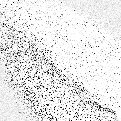
\includegraphics[width=\textwidth]{images/findings/round1/flipbook_b.png}
	\caption{After 200,000 games played}
	\end{subfigure}
	~
	\begin{subfigure}[t]{0.3\textwidth}
	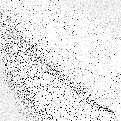
\includegraphics[width=\textwidth]{images/findings/round1/flipbook_c.png}
	\caption{After 400,000 games played}
	\end{subfigure}

	\begin{subfigure}[t]{0.3\textwidth}
	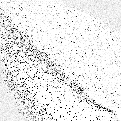
\includegraphics[width=\textwidth]{images/findings/round1/flipbook_d.png}
	\caption{After 600,000 games played}
	\end{subfigure}
	~
	\begin{subfigure}[t]{0.3\textwidth}
	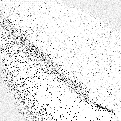
\includegraphics[width=\textwidth]{images/findings/round1/flipbook_e.png}
	\caption{After 800,000 games played}
	\end{subfigure}
	~
	\begin{subfigure}[t]{0.3\textwidth}
	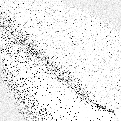
\includegraphics[width=\textwidth]{images/findings/round1/flipbook_f.png}
	\caption{Final Weights}
	\end{subfigure}

\caption{%
	Training weights representation for Agent 0's \handmaxavg\
	strategy when the agent is the dealer
	over the course of the one million games of Round 1.
	In these images, the y-axis represents the player's own score,
	the x-axis the opponent's score,
	with the origin starting at the top-left of the image.
	% N.B. This is correct of generated images from the python code
	%	as of 2018-03-08 19:12.
	% no later modifications will be made from the python code directly to
	% save myself the headache. maybe this will be converted later to be
	% more easily human understood
	% Rotate 90 deg counter-clockwise will make x=my_score, y=opp_score
}
% TODO: figure out axes
% TODO: change these images to hand_max_min: much starker contrast
\label{fig_r1-flip}
\end{figure}


\begin{figure}
\center

	\begin{subfigure}[t]{0.22\textwidth}
		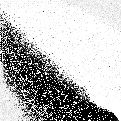
\includegraphics[width=\textwidth]{images/findings/round1/strategies_handmaxmin.png}
		\caption{\handmaxmin}
	\end{subfigure}
	~
	\begin{subfigure}[t]{0.22\textwidth}
		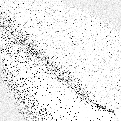
\includegraphics[width=\textwidth]{images/findings/round1/strategies_handmaxavg.png}
		\caption{\handmaxavg}
	\end{subfigure}
	~
	\begin{subfigure}[t]{0.22\textwidth}
		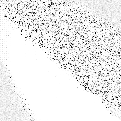
\includegraphics[width=\textwidth]{images/findings/round1/strategies_handmaxmed.png}
		\caption{\handmaxmed}
	\end{subfigure}
	~
	\begin{subfigure}[t]{0.22\textwidth}
		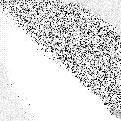
\includegraphics[width=\textwidth]{images/findings/round1/strategies_handmaxposs.png}
		\caption{\handmaxposs}
	\end{subfigure}

	\begin{subfigure}[t]{0.22\textwidth}
		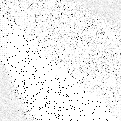
\includegraphics[width=\textwidth]{images/findings/round1/strategies_cribminavg.png}
		\caption{\cribminavg}
	\end{subfigure}
	~
	\begin{subfigure}[t]{0.22\textwidth}
		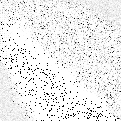
\includegraphics[width=\textwidth]{images/findings/round1/strategies_peggingmaxavggained.png}
		\caption{\peggingmaxavggained}
	\end{subfigure}
	~
	\begin{subfigure}[t]{0.22\textwidth}
		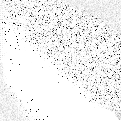
\includegraphics[width=\textwidth]{images/findings/round1/strategies_peggingmaxmedgained.png}
		\caption{\peggingmaxmedgained}
	\end{subfigure}
	~
	\begin{subfigure}[t]{0.22\textwidth}
		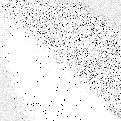
\includegraphics[width=\textwidth]{images/findings/round1/strategies_peggingminavggiven.png}
		\caption{\peggingminavggiven}
	\end{subfigure}

\caption{
	All final strategy strengths for Agent 0
	when playing as the dealer
	after training for one million games during Round 1.
}
% TODO: figure out axes
\label{fig_r1-strats}
\end{figure}

\begin{figure}
\center

	\begin{subfigure}[t]{0.22\textwidth}
		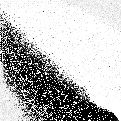
\includegraphics[width=\textwidth]{images/findings/round1/strategies_handmaxmin_pone.png}
		\caption{\handmaxmin}
	\end{subfigure}
	~
	\begin{subfigure}[t]{0.22\textwidth}
		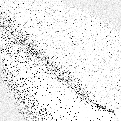
\includegraphics[width=\textwidth]{images/findings/round1/strategies_handmaxavg_pone.png}
		\caption{\handmaxavg}
	\end{subfigure}
~
	\begin{subfigure}[t]{0.22\textwidth}
		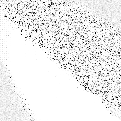
\includegraphics[width=\textwidth]{images/findings/round1/strategies_handmaxmed_pone.png}
		\caption{\handmaxmed}
	\end{subfigure}
	~
	\begin{subfigure}[t]{0.22\textwidth}
		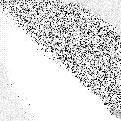
\includegraphics[width=\textwidth]{images/findings/round1/strategies_handmaxposs_pone.png}
		\caption{\handmaxposs}
	\end{subfigure}

	\begin{subfigure}[t]{0.22\textwidth}
		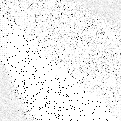
\includegraphics[width=\textwidth]{images/findings/round1/strategies_cribminavg_pone.png}
		\caption{\cribminavg}
	\end{subfigure}
	~
	\begin{subfigure}[t]{0.22\textwidth}
		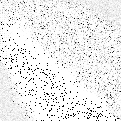
\includegraphics[width=\textwidth]{images/findings/round1/strategies_peggingmaxavggained_pone.png}
		\caption{\peggingmaxavggained}
	\end{subfigure}
~
	\begin{subfigure}[t]{0.22\textwidth}
		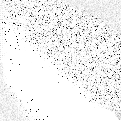
\includegraphics[width=\textwidth]{images/findings/round1/strategies_peggingmaxmedgained_pone.png}
		\caption{\peggingmaxmedgained}
	\end{subfigure}
	~
	\begin{subfigure}[t]{0.22\textwidth}
		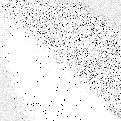
\includegraphics[width=\textwidth]{images/findings/round1/strategies_peggingminavggiven_pone.png}
		\caption{\peggingminavggiven}
	\end{subfigure}

\caption{
	All final strategy strengths for an agent
	when playing as the pone
	after training for one million games during Round 1.
}
\label{fig_r1-strats-pone}
\end{figure}



\paragraph*{Learning Results}

%%%
% Discuss Strategies Figure
%%%

%%%
Despite the all-or-nothing nature of how a single strategy is potentially
learned,
it is still worth noting that the agent did in fact learn to play different
strategies at different times.
%
As can be seen in Figure~\ref{fig_r1-strats},
the strengths of each strategy's weight do vary across score-locations.
%
For instance, when in the lead by
roughly two to twenty five points,
the agent will prefer to choose the hand with the most guaranteed
points in its own hand
by following \handmaxmin.
%
However, when the game is either extremely close
or when the agent is well in the lead,
the agent will take a slight gamble and play for expected points.
%
Occasionally, the agent will also attempt to pay attention to the points
gained through the play phase of a round by playing a combination that pegs
well.
%
Ironically,
the agent may play against its own best wishes by minimizing the average return
of the crib.
%
This is speculated to be a result of coincidental alignment of the results between
\cribminavg\ and more the reasonable \handmaxmin\
or \handmaxavg.
%%%

%%%
Of further interest is how little the agent knows about how to handle a losing
position.
%
As can be seen by looking in the upper-right half of each strategy's
individual graph,
of the explored losing states,
there is little consensus or pattern as to which strategy should dominate.
%
It is possible that agents which end up in these positions lose more often than
they win.
%
If this is the case,
the resulting punishment will decrease the top two or three strategies that were
most responsible for the hand choice at that state,
effectively increasing all others.
%
This, in turn, would likely later lead to a cycle in which different strategies
are cyclically placed in a role of strongest weight,
generating the fuzz seen now.
%%%

%%%
By comparing the pone's strategy graphs (Figure~\ref{fig_r1-strats-pone})
to those of the dealer's (Figure~\ref{fig_r1-strats}),
a few patterns emerge.
%
At first glance,
the graphs look highly similar and as if splitting up the search space into two
merely increased the complexity of finding a solution without payoff.
%
For instance,
the majority of the winning positions favor the \handmaxmin\ strategy with
a ``border'' of \handmaxavg\ being used in positions where riskier decisions
are needed or can be afforded.
%
Additionally, the losing positions offer no definitive answers and seem to be a
jumbled mess of suggestions,
the only major suggestion being to play more riskily to regain the lead.
%%%

%%%
However,
upon closer inspection,
with a side-by-side comparison,
there are subtle differences that can be found.
%
The most major of these differences is that all patterns are shifted lower and
more to the left when the agent is the dealer,
correlating with scores which are more advantageous to the player.
%
This means that the agent is more ``comfortable'' when it has a slightly larger
lead as the dealer than it necessarily needs as the pone.
%%%


%%%
% Bump/sinusoidal wave in final game stages
%		+ how they differ b/w dealer and pone
%%%

%%%
Perhaps the most interesting difference is the traceable shape of the weights
during the final scores of a close game.
%
Although difficult to discern in all but the \handmaxmin\ and \handmaxavg\ 
strategies,
the final weights trace a sinusoidal curve shape along the diagonal
for approximately the last twenty points of the game.
%
Additionally,
these waves are opposing in nature.
%
This presents the fascinating conclusion that the agent is learning
that different states or checkpoints are preferred as the player when
the dealer and when the pone.
%
Not only is this fascinating since the agent is learning a state-value function
indirectly,
but in the game of cribbage,
there exist different \textit{checkpoints} in which the player aims to get
himself by the end of a round to be in favorable position for the next.
%
Here we see evidence that the agent is learning these checkpoints throughout its
play.
%%%


\paragraph*{Performance}

%%%
% discuss how it performed worse than random (got stonked)
It is clear from the strategy graphs that,
while perhaps strategies are being over-trusted,
basic game trends are clearly being learned by the agent.
%
However, perhaps the only metric which matters from a learning perspective is
the agent's performance.
%
In this area, the learned agents failed miserably.
%
The winning agent between the two learners was pitted against
an agent using randomly allocated starting weights
where both agents would only strictly follow the policy generated
without exploration.
%
As can be seen in Table~\ref{tab_r1-randtourny},
the learned agent lost easily to the randomly-weighted agent:
with the exception of a spectacular loss in Game 3,
all other games were close losses if not wins.
%
This is speculated to be a result of the previously mentioned over-aggressive
learning pattern and its all-or-nothing end result.
%
Since the agent aligns so intensely to a single strategy,
it is not able to overcome a local optimum
and has essentially been overfit to the scenario.
%
Another potential reason for the losses could be the lack of knowledge of how to
handle losing situations.
%
As previously discussed,
in the event of a loss,
most strategies will effectively be increased except those most responsible,
contributing to a system of cycling weights.
%
Furthermore, it is also likely that an agent which finds itself in a losing
position does not end up recovering and winning the game,
meaning that
the agent effectively learns that it is mostly by chance that it will recover.
%%%

% Table to represent the tournament information

\begin{table}
\center
\begin{tabular}{|r|c|c|}
	\hline
	\textbf{Game} & \textbf{Random} & \textbf{Agent 1}\\\hline

	1 & 104 & 121 \\\hline
	2 & 121 & 114 \\\hline
	3 &  75 & 121 \\\hline
	4 & 121 & 118 \\\hline
	5 & 111 & 121 \\\hline
	6 & 121 &  99 \\\hline
	7 & 121 &  87 \\\hline
	8 & 110 & 121 \\\hline
	9 & 121 &  64 \\\hline

\end{tabular}
~
\begin{tabular}{|r|c|c|c|}
	\hline
	\textbf{Agent} & \textbf{Score} & \textbf{Point Spread} & \textbf{Wins}
	\\\hline
	Random & 12 & +39 & 5
	\\\hline
	Agent 1 & 9 & \textemdash & 4
	\\\hline
\end{tabular}

\label{tab:r1-randtourny}

\caption{
	Results of a nine-game tournament played between
	a randomly-weighted agent
	and
	Agent 1 after learning for one million games.
}

\end{table}


%%%
% discussion of playing an agent against a previous version of itself
%%%

%%%
In order to more accurately diagnose if an overfitting situation was occurring,
a winning agent was played against its own previous checkpoints.
%
A sample set of scores can be found in Table~\ref{tab_r1-selftourny}.
%
The point spreads from twenty separate 100-game tournaments
are depicted in Figure~\ref{fig_r1-spreads_a}.
%
While point spreads are from total points pegged to the board,
not gained from wins
and therefore not a direct indicator of performance in tournament play,
it is useful for determining general performance.
%
Furthermore,
point spreads are the parameters used for direct feedback as the rewards
during the training phase,
so it is a direct indicator of learning the task for which it was trained.
%
As can be seen, there is no discernible correlation or pattern between
epoch checkpoint and performance.
%
This indicates that,
despite a policy being learned,
quite a lot is still left to chance of the cards dealt.
%
This has the potential to be exacerbated even further when policies are nearly
deterministic and non-adaptive in their weight assignments.
%
Additionally,
a random agent was played against its future iterations in the same fashion,
with the similar results, not shown. % depicted in Table~\ref{tab_r1-spreads_b}.
%%%


% Table of results for an agent against itself

 % TODO: fill in with actual data

\begin{table}
\center

\begin{tabular}{|r|c|c|c|}
	\hline
	\textbf{Epochs} & \textbf{Score} & \textbf{Spread} & \textbf{Wins}
	\\\hline
	0 & 126 & +523 & 59
	\\\hline
	1MM & 86 & \textemdash & 41
	\\\hline
\end{tabular}
~
\begin{tabular}{|r|c|c|c|}
	\hline
	\textbf{Epochs} & \textbf{Score} & \textbf{Spread} & \textbf{Wins}
	\\\hline
	100K & 122 & +200 & 55
	\\\hline
	1MM & 104 & \textemdash & 45
	\\\hline
\end{tabular}

\begin{tabular}{|r|c|c|c|}
	\hline
	\textbf{Epochs} & \textbf{Score} & \textbf{Spread} & \textbf{Wins}
	\\\hline
	200K & 108 & -27 & 47
	\\\hline
	1MM & 118 & \textemdash & 53
	\\\hline
\end{tabular}
~
\begin{tabular}{|r|c|c|c|}
	\hline
	\textbf{Epochs} & \textbf{Score} & \textbf{Spread} & \textbf{Wins}
	\\\hline
	300K & 105 & -180 & 48
	\\\hline
	1MM & 116 & \textemdash & 52
	\\\hline
\end{tabular}

\begin{tabular}{|r|c|c|c|}
	\hline
	\textbf{Epochs} & \textbf{Score} & \textbf{Spread} & \textbf{Wins}
	\\\hline
	400K & 87 & -510 & 41
	\\\hline
	1MM & 133 & \textemdash & 59
	\\\hline
\end{tabular}
~
\begin{tabular}{|r|c|c|c|}
	\hline
	\textbf{Epochs} & \textbf{Score} & \textbf{Spread} & \textbf{Wins}
	\\\hline
	500K & 97 & -386 & 43
	\\\hline
	1MM & 129 & \textemdash & 57
	\\\hline
\end{tabular}

\begin{tabular}{|r|c|c|c|}
	\hline
	\textbf{Epochs} & \textbf{Score} & \textbf{Spread} & \textbf{Wins}
	\\\hline
	600K & 117 & 370 & 52
	\\\hline
	1MM & 98 & \textemdash & 48
	\\\hline
\end{tabular}
~
\begin{tabular}{|r|c|c|c|}
	\hline
	\textbf{Epochs} & \textbf{Score} & \textbf{Spread} & \textbf{Wins}
	\\\hline
	700K & 107 & -174 & 48
	\\\hline
	1MM & 115 & \textemdash & 52
	\\\hline
\end{tabular}

\begin{tabular}{|r|c|c|c|}
	\hline
	\textbf{Epochs} & \textbf{Score} & \textbf{Spread} & \textbf{Wins}
	\\\hline
	800K & 124 & 239 & 56
	\\\hline
	1MM & 96 & \textemdash & 44
	\\\hline
\end{tabular}
~
\begin{tabular}{|r|c|c|c|}
	\hline
	\textbf{Epochs} & \textbf{Score} & \textbf{Spread} & \textbf{Wins}
	\\\hline
	900K & 111 & -82 & 51
	\\\hline
	1MM & 111 & \textemdash & 49
	\\\hline
\end{tabular}


%%%%%%%%
%
%\begin{tabular}{|r|c|c|c|}
%	\hline
%	\textbf{Epochs} & \textbf{Score} & \textbf{Spread} & \textbf{Wins}
%	\\\hline
%	100K & 104 & -108 & 50
%	\\\hline
%	1MM & 111 & \textemdash & 50
%	\\\hline
%\end{tabular}
%~
%\begin{tabular}{|r|c|c|c|}
%	\hline
%	\textbf{Epochs} & \textbf{Score} & \textbf{Spread} & \textbf{Wins}
%	\\\hline
%	250K & 104 & -268 & 47
%	\\\hline
%	1MM & 121 & \textemdash & 53
%	\\\hline
%\end{tabular}
%
%~
%
%\begin{tabular}{|r|c|c|c|}
%	\hline
%	\textbf{Epochs} & \textbf{Score} & \textbf{Spread} & \textbf{Wins}
%	\\\hline
%	500K & 104 & -116 & 49
%	\\\hline
%	1MM & 109 & \textemdash & 51
%	\\\hline
%\end{tabular}
%~
%\begin{tabular}{|r|c|c|c|}
%	\hline
%	\textbf{Epochs} & \textbf{Score} & \textbf{Spread} & \textbf{Wins}
%	\\\hline
%	750K & 113 & +33 & 53
%	\\\hline
%	1MM & 104 & \textemdash & 47
%	\\\hline
%\end{tabular}

\label{tab:r1-selftourny}

\caption{
	Results of multiple 100-game tournaments played between
	agents using various epoch checkpoints from the training
	and the final agent from the round.
	The weights used here are from Agent 1.
}

\end{table}


% Point spreads for two runs of blah

\begin{figure}
\center

\begin{subfigure}[b]{0.8\textwidth}
	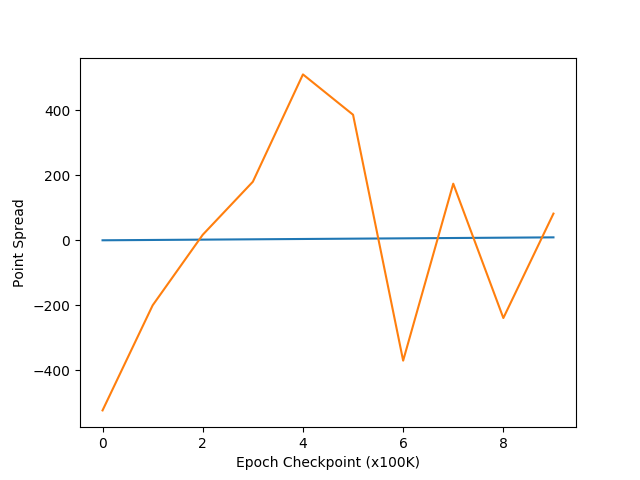
\includegraphics[width=\linewidth]{images/findings/round1/spread1.png}
	\label{fig_r1-spreads_a}
	\caption{}
\end{subfigure}

\begin{subfigure}[b]{0.8\textwidth}
	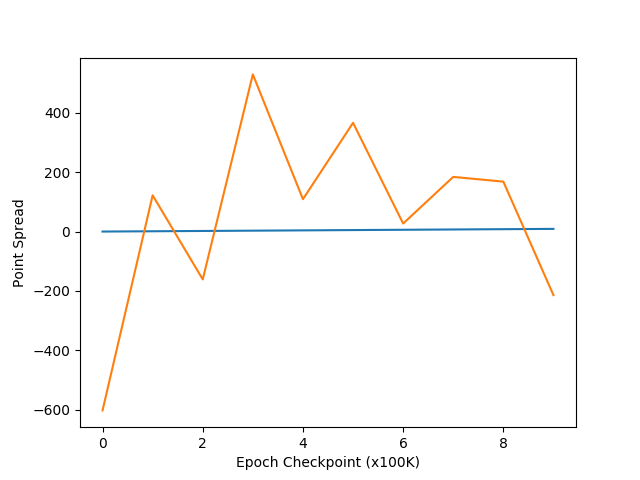
\includegraphics[width=\linewidth]{images/findings/round1/spread2.png}
	\label{fig_r1-spreads_b}
	\caption{}
\end{subfigure}

\caption{
	Point spreads across two 100-game tournaments pitting a winning
	agent against its checkpoints.
	Here, a positive point spread indicates that the fully-trained agent has
	accumulated more points than its opponent,
	an agent created from a checkpoint generated after the number of training
	game epochs indicated on the x-axis.
}
\label{fig_r1-spreads}
\end{figure}



\paragraph*{Applications for Round 2}

%%%
% "Lessons Learned" / changes made
%	Learning rate lowered
%	exploration rate constant
%	trained random v learning in order to learn the game
%%%

%%%
% discuss how the meta-parameters were tweaked for round 2
%		and how the tournament structure got wonked
%%%

%%%
As a result of the presumed over-aggressive learning of single strategies,
some learning parameters were altered for Round 2.
%
Since it was estimated to be the primary reason for the learning behavior,
the first parameter adjustment made was to decrease the learning rate drastically.
%
The learning rate was decreased to one fifth of what was used in Round 1.
%
The other major parameter alteration was to make the exploration rate a constant
and not dependent upon the variance of the weights.
%
During Round 1,
the exploration rate was defined as $e = 0.3 - \Var({w_{p,o,d}})$
in order to allow more trained states to be less affected by randomized
exploration.
%
As a result,
the most strongly biased weight locations would only allow for exploration
even more rarely than before.
%
Although only producing a decrease from a 30\% chance to 18\%,
this would still result in a smaller likelihood of exploring in the current 
state,
potentially further cementing of the dominant strategy in its position.
%
Additionally,
it was a complication which, upon further thought, would not result in much
difference over the course of time
and thus deemed non-beneficial and ultimately unnecessary.
%%%

%%%
% tournament structure
%%%

%%%
In order to see if the heavily biased weights could be tempered down to more
reasonable mixes which could outplay a random agent,
the structure of the tournament was updated.
%
In addition to having the winners of the previous pair of agents square
off against one another,
there was a ``loser's bracket'' created
in which the losers would start over from ground zero.
%
These two ways of playing were intended as a two-pronged approach
in order to see if multiple agents could be trained at the same time
which could outperform random.
%
The ``winners bracket'' would determine if a highly-biased set of agents could
learn nuance
while the ``losers bracket'' would test if it were possible for two constantly
competing agents could ever actually increase performance when both are each
updating their parameters to combat each other.
%%%

%%%
% random v learning
%	two agents paired with two random agents
%	one learns, other stays the same. learns game, not how to outmatch opponent
%%%

%%%
Since the agents were assumed to be learning how to outplay each other
but not the game,
the next phase would attempt to determine the extent of this tailored learning.
%
In addition to the previously mentioned alterations to the tournament structure,
a new batch of agents would be trained against a static, entirely random agent.
%
Rather than both agents in the game learning and altering their weights after
each game,
only one agent would train its weights.
%
The prevailing logic behind this decision was that if each agent was indirectly
affecting the other,
the environment could be said to be slightly altered.
%
This would, in turn, mean that the agents are no longer learning the original
problem.
%%%



% Round 2 findings section

\subsubsection*{Round 2}
\label{sec:findings-r2}

\paragraph*{Performance}
\label{sec:findings-r2-perf}

%%%
% TODO: Discussion of performance
%%%

%%%
Judging by the lack of pattern found in
Figures~\ref{fig:r2-spreads-winner},
\ref{fig:r2-spreads-loser},
and~\ref{fig:r2-spreads-random},
there is no significant performance increase to be found from Round 2.
%
If learning had occurred,
Figures~\ref{fig:r2-spreads-winner-a},
\ref{fig:r2-spreads-loser-a},
and~\ref{fig:r2-spreads-random-a}
would take on the form of a decreasing curve,
gradually approaching zero,
while Figures~\ref{fig:r2-spreads-winner-b},
\ref{fig:r2-spreads-loser-b},
and~\ref{fig:r2-spreads-random-b}
would be their mirror across the x-axis.
%
Figure~\ref{fig:r2-spreads-winner} alone
would indicate that an agent trained for one million games plays on par with
one trained for two million games.
%
On its own,
this would indicate that performance had reached a peak and saturated.
%
However,
the similarity to Figure~\ref{fig:r2-spreads-loser}
and even Figure~\ref{fig:r2-spreads-random}
show that neither bracket learned to perform better than previous iterations.
%%%

% Point spreads for two runs of blah

\begin{figure}
\center

\begin{subfigure}[b]{0.45\textwidth}
	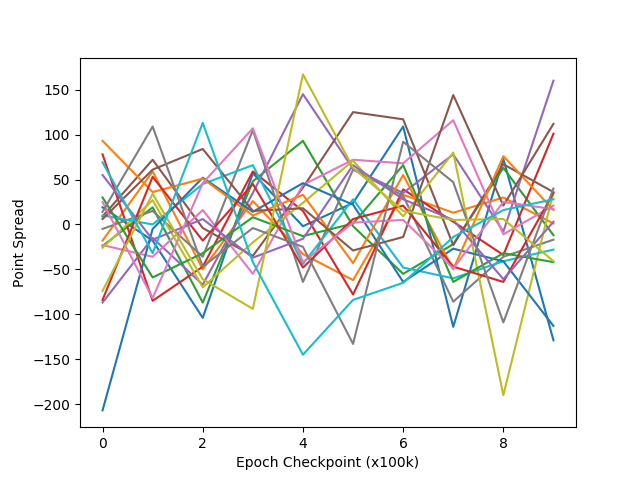
\includegraphics[width=\linewidth]{images/findings/round2/spreads_self-v-prev_winner.png}
	\caption{An agent plays against previous iterations of itself.}
	\label{fig:r2-spreads-winner-a}
\end{subfigure}
~
\begin{subfigure}[b]{0.45\textwidth}
	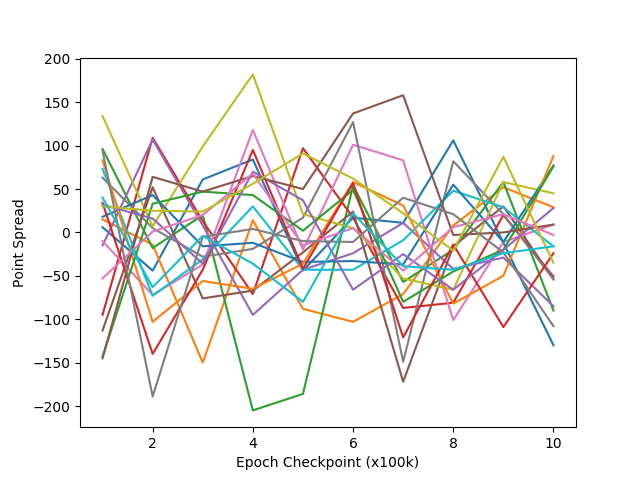
\includegraphics[width=\linewidth]{images/findings/round2/spreads_rand-v-fut_winner.png}
	\caption{A random agent plays against later, more learned agents.}
	\label{fig:r2-spreads-winner-b}
\end{subfigure}

\caption{
	Point spreads across twenty 9-game tournaments for an agent in the
	winners' bracket of Round 2.
	Note that since the winners' bracket uses an agent with prior training,
	the total epochs elapsed is one million more than displayed.
}
\label{fig:r2-spreads-winner}
\end{figure}


% Point spreads for two runs of blah

\begin{figure}
\center

\begin{subfigure}[b]{0.45\textwidth}
	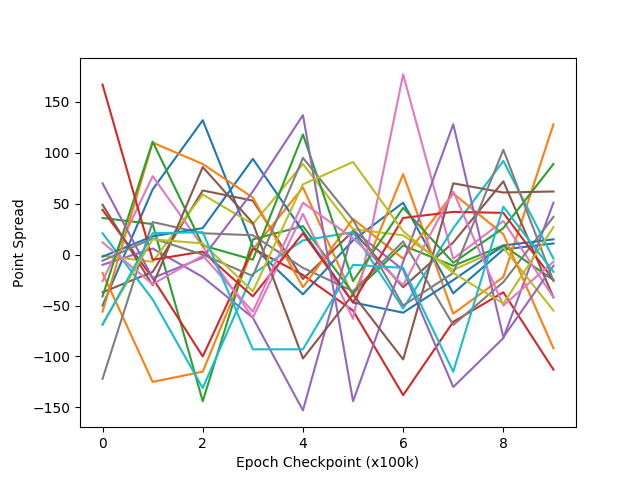
\includegraphics[width=\linewidth]{images/findings/round2/spreads_self-v-prev_loser.png}
	\caption{An agent plays against previous iterations of itself.}
	\label{fig:r2-spreads-loser-a}
\end{subfigure}
~
\begin{subfigure}[b]{0.45\textwidth}
	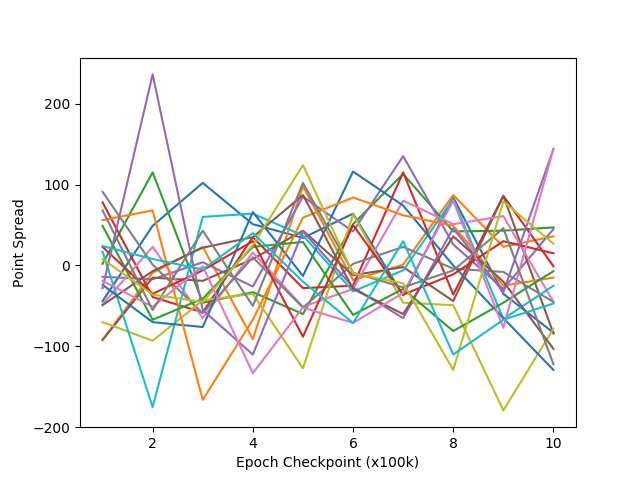
\includegraphics[width=\linewidth]{images/findings/round2/spreads_rand-v-fut_loser.png}
	\caption{A random agent plays against later, more learned agents.}
	\label{fig:r2-spreads-loser-b}
\end{subfigure}

\caption{
	Point spreads across mutliple 9-game tournamens of an agent in the
	losers' bracket of Round 2.
}
\label{fig:r2-spreads-loser}
\end{figure}


\begin{figure}
\center

%\includegraphics[width=0.8\textwidth]{images/findings/round2/spreads_random.png}
\begin{subfigure}[b]{0.90\textwidth}
	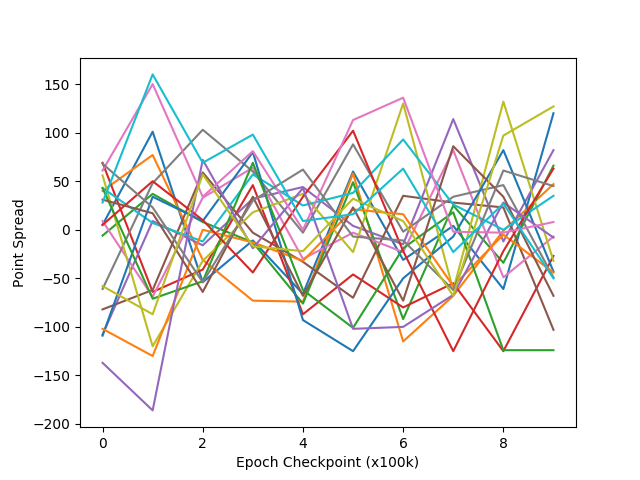
\includegraphics[width=\linewidth]{images/findings/round2/spreads_self-v-prev_random.png}
	\caption{An agent plays against previous iterations of itself.}
	\label{fig:r2-spreads-random-a}
\end{subfigure}

\begin{subfigure}[b]{0.90\textwidth}
	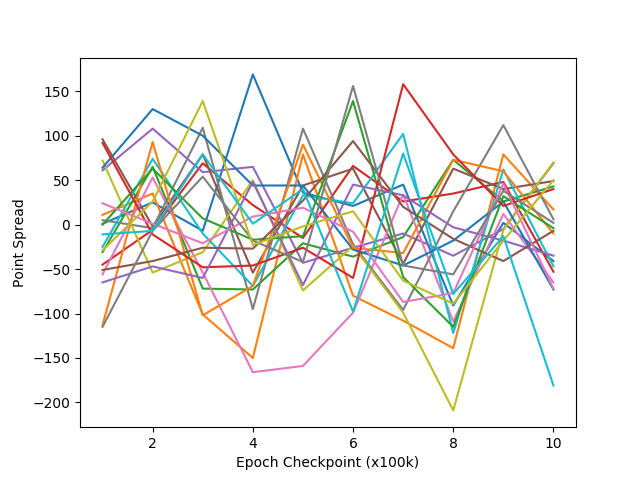
\includegraphics[width=\linewidth]{images/findings/round2/spreads_rand-v-fut_random.png}
	\caption{A random agent plays against later, more learned agents.}
	\label{fig:r2-spreads-random-b}
\end{subfigure}


\caption{
	Point spreads across mutliple 9-game tournamens of an agent
	trained against a static, unlearning agent with random weights.
}
\label{fig:r2-spreads-random}
\end{figure}




\paragraph*{Learning Process and Results}
\label{sec:findings-r2-results}

%%%
% Discussion of what it learns and why that's interesting from a cribbage
% perspective
%%%


\begin{figure}
\center

	\begin{subfigure}[t]{0.22\textwidth}
		
\includegraphics[width=\textwidth]{images/findings/round2/strats/winner/hand_max_min.png}
		\caption{\handmaxmin}
	\end{subfigure}
	~
	\begin{subfigure}[t]{0.22\textwidth}
		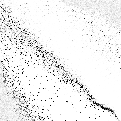
\includegraphics[width=\textwidth]{images/findings/round2/strats/winner/hand_max_avg.png}
		\caption{\handmaxavg}
	\end{subfigure}
	~
	\begin{subfigure}[t]{0.22\textwidth}
		
\includegraphics[width=\textwidth]{images/findings/round2/strats/winner/hand_max_med.png}
		\caption{\handmaxmed}
	\end{subfigure}
	~
	\begin{subfigure}[t]{0.22\textwidth}
		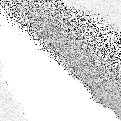
\includegraphics[width=\textwidth]{images/findings/round2/strats/winner/hand_max_poss.png}
		\caption{\handmaxposs}
	\end{subfigure}

	\begin{subfigure}[t]{0.22\textwidth}
		
\includegraphics[width=\textwidth]{images/findings/round2/strats/winner/crib_min_avg.png}
		\caption{\cribminavg}
	\end{subfigure}
	~
	\begin{subfigure}[t]{0.22\textwidth}
		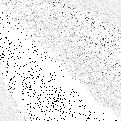
\includegraphics[width=\textwidth]{images/findings/round2/strats/winner/pegging_max_avg_gained.png}
		\caption{\peggingmaxavggained}
	\end{subfigure}
	~
	\begin{subfigure}[t]{0.22\textwidth}
		
\includegraphics[width=\textwidth]{images/findings/round2/strats/winner/pegging_max_med_gained.png}
		\caption{\peggingmaxmedgained}
	\end{subfigure}
	~
	\begin{subfigure}[t]{0.22\textwidth}
		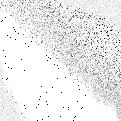
\includegraphics[width=\textwidth]{images/findings/round2/strats/winner/pegging_min_avg_given.png}
		\caption{\peggingminavggiven}
	\end{subfigure}

\caption{
	All final strategy strengths for an agent in the winners' bracket
	when playing as the dealer
	after training for one million games during Round 1
	and a further one million games during Round 2.
}
\label{fig:r2-strats-winner}
\end{figure}


%%%
Despite the lack of performance increase after another million games played by
both the winning and losing brackets,
there are still interesting trends to be spotted between the different brackets
of play.
%
The most notable is how quickly policies converge to a similar state.
%
While the strategy graphs for the less trained agents are less ``crisp''
in their appearance thanks to their slower learning rates,
the patterns of which policy to mainly follow at which times
are still quick to form.
%
% TODO: vvv do we want to mention this at all? what purpose does it serve?
This is useful because it allows for the possibility of running future
experiments with fewer training epochs in less time.
%
This, in turn, allows for a larger variety of methods to be tested to improve
the cribbage-playing agent.
%%%

%%%
Even more fascinating observations can be found from the strategy graphs
from the winner's bracket (see Figure~\ref{r2-strats-winner}).
%
By focusing on the \handmaxmin\ and \handmaxavg\ strategies in particular,
the sinusoidal wave along the diagonal can be observed extending further
back along the diagonal to earlier game positions,
albeit with smaller amplitude.
%
While not being of much use to the agent directly,
this is a useful observation from a cribbage player's perspective.
%
Since it is possible to infer the state-value function,
the implications of this wave are that earlier states are not crucial
predictors for future success.
%
Not only that,
but the agent has learned that changes in lead are likely and not necessarily
detrimental to the ability to win the game.
%%%

%%%
Care needs to be taken with this previous observation on the wave's amplitude
and it must be pointed out to be speculation on the part of the author.
%
It may be the case that with enough training the sine wave will be at full
amplitude in earlier positions.
%
A reminder must be made that
a notable reason for the lack of clarity at the moment is the weight adjustment
mechanism for training.
%
The training system pre-supposes that the earlier positions are of less
importance in a game and adjusts them with a lower priority than later positions
in the game.
%
It may indeed be the case that two million games is still not enough to
counteract the decay of temporal difference learning with the learning
rate used.
%%%


%%%
% Talking about loser's bracket and how it compares to winner's
%%%


\begin{figure}
\center

	\begin{subfigure}[t]{0.22\textwidth}
		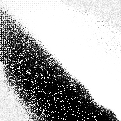
\includegraphics[width=\stratgraphwidth]{images/findings/round2/strats/loser/hand_max_min.png}
		\caption{\handmaxmin}
	\end{subfigure}
	~
	\begin{subfigure}[t]{0.22\textwidth}
		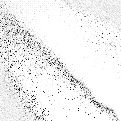
\includegraphics[width=\stratgraphwidth]{images/findings/round2/strats/loser/hand_max_avg.png}
		\caption{\handmaxavg}
	\end{subfigure}
	~
	\begin{subfigure}[t]{0.22\textwidth}
		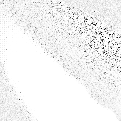
\includegraphics[width=\stratgraphwidth]{images/findings/round2/strats/loser/hand_max_med.png}
		\caption{\handmaxmed}
	\end{subfigure}
	~
	\begin{subfigure}[t]{0.22\textwidth}
		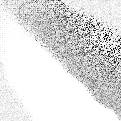
\includegraphics[width=\stratgraphwidth]{images/findings/round2/strats/loser/hand_max_poss.png}
		\caption{\handmaxposs}
	\end{subfigure}

	\begin{subfigure}[t]{0.22\textwidth}
		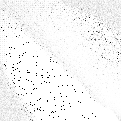
\includegraphics[width=\stratgraphwidth]{images/findings/round2/strats/loser/crib_min_avg.png}
		\caption{\cribminavg}
	\end{subfigure}
	~
	\begin{subfigure}[t]{0.22\textwidth}
		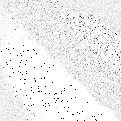
\includegraphics[width=\stratgraphwidth]{images/findings/round2/strats/loser/pegging_max_avg_gained.png}
		\caption{\peggingmaxavggained}
	\end{subfigure}
	~
	\begin{subfigure}[t]{0.22\textwidth}
		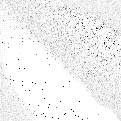
\includegraphics[width=\stratgraphwidth]{images/findings/round2/strats/loser/pegging_max_med_gained.png}
		\caption{\peggingmaxmedgained}
	\end{subfigure}
	~
	\begin{subfigure}[t]{0.22\textwidth}
		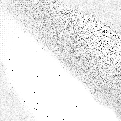
\includegraphics[width=\stratgraphwidth]{images/findings/round2/strats/loser/pegging_min_avg_given.png}
		\caption{\peggingminavggiven}
	\end{subfigure}

\caption{
	All final strategy strengths for an agent in the losers' bracket
	when playing as the dealer
	after training for one million games during Round 2.
}
\label{fig:r2-strats-loser}
\end{figure}


%%%
By comparing the winner's bracket strategy graphs to those of the loser's
bracket,
a vast degree of similarity can be found.
%
In both brackets,
the same behavioral trends are learned.
%
However,
there does exist a small amount of difference between the two
in how quickly and surely each trend is learned.
%
The winner's bracket mostly reinforces its current weight choices
with the losing triangle becoming slightly gradiented.
Meanwhile,
in the loser's bracket,
the gradient applies more evenly to the entire range of strategies
across the winning-losing boundary.
%
Of additional note,
there are fewer spaces in which
strategies such as \cribminavg, \peggingmaxavggained, and \peggingminavggiven\ 
have been strengthened within the \handmaxmin\ \textit{block}.
%
This is a good indicator that,
although present,
there is less of a bias towards those strategies which are initially winners.
%%%


\begin{figure}
\center

	\begin{subfigure}[t]{0.22\textwidth}
		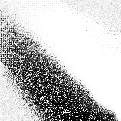
\includegraphics[width=\stratgraphwidth]{images/findings/round2/strats/random/hand_max_min.png}
		\caption{\handmaxmin}
	\end{subfigure}
	~
	\begin{subfigure}[t]{0.22\textwidth}
		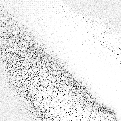
\includegraphics[width=\stratgraphwidth]{images/findings/round2/strats/random/hand_max_avg.png}
		\caption{\handmaxavg}
	\end{subfigure}
	~
	\begin{subfigure}[t]{0.22\textwidth}
		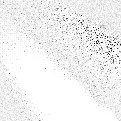
\includegraphics[width=\stratgraphwidth]{images/findings/round2/strats/random/hand_max_med.png}
		\caption{\handmaxmed}
	\end{subfigure}
	~
	\begin{subfigure}[t]{0.22\textwidth}
		\includegraphics[width=\stratgraphwidth]{images/findings/round2/strats/random/hand_max_poss.png}
		\caption{\handmaxposs}
	\end{subfigure}

	\begin{subfigure}[t]{0.22\textwidth}
		\includegraphics[width=\stratgraphwidth]{images/findings/round2/strats/random/crib_min_avg.png}
		\caption{\cribminavg}
	\end{subfigure}
	~
	\begin{subfigure}[t]{0.22\textwidth}
		\includegraphics[width=\stratgraphwidth]{images/findings/round2/strats/random/pegging_max_avg_gained.png}
		\caption{\peggingmaxavggained}
	\end{subfigure}
	~
	\begin{subfigure}[t]{0.22\textwidth}
		\includegraphics[width=\stratgraphwidth]{images/findings/round2/strats/random/pegging_max_med_gained.png}
		\caption{\peggingmaxmedgained}
	\end{subfigure}
	~
	\begin{subfigure}[t]{0.22\textwidth}
		\includegraphics[width=\stratgraphwidth]{images/findings/round2/strats/random/pegging_min_avg_given.png}
		\caption{\peggingminavggiven}
	\end{subfigure}

\caption{
	All final strategy strengths for a learning agent
	after playing a completely random agent
	when playing as the pone
	after training for 350,000 games during Round 2.
}
\label{fig:r2-strats-random}
\end{figure}


%%%
% TODO: discuss random tourny's stuff
%%%

%%%
In analyzing the evolution of the \handmaxavg\ strategy in both the winner's
and loser's brackets,
it can clearly be seen that the general trend of behavior forms
relatively quickly,
i.e. after the first half million games played.
%
Beyond that amount of games,
the agent learns to refine the strategy boundaries,
but it can be said that there is little discovery being made.
%
This is useful because it allows for quicker training rounds to be played,
and thus more possible variations in training can be tried in the time given
with the goal of improving beyond random play.
%%%


% Figure for the flipbook of strategies over time

\begin{figure}
\center

	\begin{subfigure}[t]{0.2\textwidth}
	\includegraphics[width=\textwidth]{images/findings/round2/flipbook/loser/checkpoint_000000.png}
	\caption{Starting Weights}
	\end{subfigure}
	~
	\begin{subfigure}[t]{0.2\textwidth}
	\includegraphics[width=\textwidth]{images/findings/round2/flipbook/loser/checkpoint_200000.png}
	\caption{After 200,000 games played}
	\end{subfigure}
	~
	\begin{subfigure}[t]{0.2\textwidth}
	\includegraphics[width=\textwidth]{images/findings/round2/flipbook/loser/checkpoint_400000.png}
	\caption{After 400,000 games played}
	\end{subfigure}

	\begin{subfigure}[t]{0.2\textwidth}
	\includegraphics[width=\textwidth]{images/findings/round2/flipbook/loser/checkpoint_600000.png}
	\caption{After 600,000 games played}
	\end{subfigure}
	~
	\begin{subfigure}[t]{0.2\textwidth}
	\includegraphics[width=\textwidth]{images/findings/round2/flipbook/loser/checkpoint_800000.png}
	\caption{After 800,000 games played}
	\end{subfigure}
	~
	\begin{subfigure}[t]{0.2\textwidth}
	\includegraphics[width=\textwidth]{images/findings/round2/flipbook/loser/checkpoint_999999.png}
	\caption{Final Weights}
	\end{subfigure}

\caption{
	Training weights representation for a losers' bracket agent's \handmaxavg\
	strategy when the agent is the dealer
	over the course of the one million games of Round 2.
}
\label{fig:r2-flip-loser}
\end{figure}


% Figure for the flipbook of strategies over time

\begin{figure}
\center

	\begin{subfigure}[b]{0.4\textwidth}
	\includegraphics[width=\linewidth]{images/findings/round2/flipbook/winner/checkpoint_000000.png}
	\caption{Starting Weights}
	\end{subfigure}
	~
	\begin{subfigure}[b]{0.4\textwidth}
	\includegraphics[width=\linewidth]{images/findings/round2/flipbook/winner/checkpoint_200000.png}
	\caption{After 200,000 games played}
	\end{subfigure}

	\begin{subfigure}[b]{0.4\textwidth}
	\includegraphics[width=\linewidth]{images/findings/round2/flipbook/winner/checkpoint_400000.png}
	\caption{After 400,000 games played}
	\end{subfigure}
	~
	\begin{subfigure}[b]{0.4\textwidth}
	\includegraphics[width=\linewidth]{images/findings/round2/flipbook/winner/checkpoint_600000.png}
	\caption{After 600,000 games played}
	\end{subfigure}

	\begin{subfigure}[b]{0.4\textwidth}
	\includegraphics[width=\linewidth]{images/findings/round2/flipbook/winner/checkpoint_800000.png}
	\caption{After 800,000 games played}
	\end{subfigure}
	~
	\begin{subfigure}[b]{0.4\textwidth}
	\includegraphics[width=\linewidth]{images/findings/round2/flipbook/winner/checkpoint_999999.png}
	\caption{Final Weights}
	\end{subfigure}

\caption{
	Training weights representation for a winner bracket agent's \handmaxavg\
	strategy when the agent is the dealer
	over the course of the one million games of Round 2.
	Note that the starting weights are carried over from Round 1,
	so the total training epochs to reach each position is actually
	one million higher than expressed.
}
\label{fig:r2-flip-winner}
\end{figure}


% Figure for the flipbook of strategies over time

\begin{figure}
\center

	\begin{subfigure}[b]{0.4\textwidth}
	\includegraphics[width=\linewidth]{images/findings/round2/flipbook/random/checkpoint_000000.png}
	\caption{Starting Weights}
	\end{subfigure}
	~
	\begin{subfigure}[b]{0.4\textwidth}
	\includegraphics[width=\linewidth]{images/findings/round2/flipbook/random/checkpoint_200000.png}
	\caption{After 200,000 games played}
	\end{subfigure}

	\begin{subfigure}[b]{0.4\textwidth}
	\includegraphics[width=\linewidth]{images/findings/round2/flipbook/random/checkpoint_400000.png}
	\caption{After 400,000 games played}
	\end{subfigure}
	~
	\begin{subfigure}[b]{0.4\textwidth}
	\includegraphics[width=\linewidth]{images/findings/round2/flipbook/random/checkpoint_600000.png}
	\caption{After 600,000 games played}
	\end{subfigure}

	\begin{subfigure}[b]{0.4\textwidth}
	\includegraphics[width=\linewidth]{images/findings/round2/flipbook/random/checkpoint_800000.png}
	\caption{After 800,000 games played}
	\end{subfigure}
	~
	\begin{subfigure}[b]{0.4\textwidth}
	\includegraphics[width=\linewidth]{images/findings/round2/flipbook/random/checkpoint_999999.png}
	\caption{Final Weights}
	\end{subfigure}

\caption{
	Training weights representation for a winner bracket agent's \handmaxavg\
	strategy when the agent is the dealer
	over the course of the one million games of Round 2.
}
\label{fig:r2-flip-random}
\end{figure}



%%%
% Section on why the hell nothing seems to work (speculation)
%%%


\paragraph*{Potential Issues}
\label{sec:findings-r2-potentialissues}

%%%
Before modifications can be made to the learning framework,
the comparable performance to random weights must first be addressed as a potential
error in implementation rather than in training.
%
Since all methods of training so far have resulted in very similar policies
being learned,
it is fair to say that policy learned during training has been superior to
random in some manner.
%
There are then a couple items to consider with regard to why such poor results are occurring
during the review tournaments,
such as the scale of play and potential overfitting of the model.
%%%


%%%\subparagraph*{Overfitting}
%%%
%%%%%%
%%%% Overfitting
%%%The first item to consider as the source of the discrepancy between the
%%%observation that a policy is learned,
%%%but its performance is abysmal,
%%%is that the weights table is overfitting to the problem.
%%%%
%%%This would have been especially true of the first round where learning rates
%%%were much higher.
%%%%
%%%However,
%%%if the agents were to be overfitting,
%%%a number of differences would be found in their results.
%%%%
%%%Firstly,
%%%a different set of policy graphs would likely result from the training phase,
%%%which is not the case.
%%%%
%%%More importantly,
%%%a definitive curve would be present in the tournament graphs as performance
%%%would increase before dropping.
%%%%
%%%As can be seen in Figure~\ref{fig:r2-time-series},
%%%this is not the case
%%%as performance is not apparently linked to training in any way.
%%%%
%%%Therefore, it would seem safe to conclude that overfitting is not the reason
%%%for the poor resulting performance.
%%%%%%


\subparagraph*{Scale of Play}

%%%
The prevailing theory as to the reason for which the agent learns a policy,
but following that policy does not yield positive results in performance,
is the issue of scale.
%
The agent is trained on a million games,
but tested on only a handful.
%
Since the cards being dealt are not taken into account by the policy,
the decisions made will likely be inaccurate on the scale of a single game,
but not for thousands.
%%%

% Figures
\input{sections/findings/round2/r2-time-series.fig.tex}
% /Figures

%%%
% Discussion of how scale affects score spreads
%	On 9-game scale, we have utter chaos, maybe not worth mentioning?
%	On 100-game scale, utter chaos
%	On 1000-game scale, maybe a little, if we squint hard,
%	On 10k-game scale, we can see a pattern
%		contradicts the 1k-game observations
%		consistently even with random
%		sharp increase in performance over 100k-200k
%		even play for the next 600k
%		seemingly regain advantage in the last 200k
%%%

%%%
A regulation cribbage match between two human players consists of nine games.
%
As can be seen in Figure~\ref{fig:r2-time-series-100},
in a series of 100-game matches between a fully trained agent and its
previous checkpoints\textemdash
using a Round 2-trained agent in the losers' bracket for demonstrative
purposes\textemdash
no pattern is discernible in total point spreads between the two playing agents.
%
This demonstrates that,
on this scale,
the winner of the game is no more predictable than a truly random coin toss.
%%%

%%%
When the scale is increased to one thousand games,
a slight pattern begins to emerge
when visualized in Figure~\ref{fig:r2-time-series-1000}.
%
Whereas the majority of the graph remains highly varying and unpatterned,
the first few games begin to trace a common curve.
%
The match against the random agent is still unpredictable,
but the matches against the 100,000 and 200,000 game trained checkpoints are
consistently beaten by the final agent.
%%%

%%%
Although fewer matches are played to compensate for the additional time needed to
play the increased number of games,
the same pattern beginning to form in the thousand-game scale is visible in the
ten thousand-game matches.
%
With the exception of the purely untrained agent,
the least \learned\ agents perform the poorest against the final
\learned\ agent.
%
Play is approximately evenly matched between the fully trained agent
and its checkpoints which have been trained for 300,000 to 700,000 games.
%
Following these matches,
the agent begins to, again, win more consistently when more training is done.
%
This confusingly indicates that more recent agents are getting worse
than earlier iterations,
yet the final agent is better than these.
%
The reasons for this trend are unknown.
%%%

\subparagraph*{Overfitting}

%%%
If the agent is being trained correctly and no overfitting is occurring,
then the point spread should be a positive number,
gradually decreasing and approaching zero
as more training is applied to its opponent,
forming a similar curve to a loss metric used in classical machine learning.
%
In the event of overfitting,
the curve would dip below the zero before reapproaching zero.
%
Neither of these shapes were seen in the resulting graph
(Figure~\ref{fig:r2-time-series-10000}).
%
Instead,
the shape of the curve implies that,
since the random agent performs consistently better than the trained agent,
the learning process is not learning the game so much as how to outplay
or edge out its
opponent in some experienced scenarios that do not
generalize to the testing phase.
%reappear during testing.
%
This conclusion is supported by the observation that the agents with limited
training are steadfastly outplayed.
%%%

%%%
Also of further note, is the scale on the aforementioned graphs.
%
In Figure~\ref{fig:r2-time-series-10000},
the maximum point spread achieved is just a shade above 10,000 points
over the course of 10,000 games.
%
This means that the average point spread advantage is approximately 
one point per game at peak performance\textemdash
and most often $0.2$ points per game\textemdash
in long-term play.
%
The average spread increases to about $30$ points per game when fewer games are 
played,
but since performance is unpredictable on this scale,
this can be explained as a result of the randomness of the cards given
and cannot be considered a reliable measure of performance.
%%%%
%%%In fact,
%%%in sampled matches,
%%%it was not uncommon to observe losses and wins of 30 points or more
%%%as well as much closer games with margins of only a few points.
%
In addition to the randomness of cards dealt,
this massive point sway could also be the result of the agents' uncertainty on 
how to recover from a losing position.
%
While the reasons for this inability cannot be said to be more than speculation,
the learning of a policy directly, without taking into account cards dealt,
is the likely culprit,
as explained previously.
%%%






%%%
% Any results of the experimental runs
%%%

\subsection{Further Experiments}
\label{sec:findings-expts}

%%%
As the results of Round 2 emulated those of Round 1,
the tournament structure was abandoned and
additional modifications were made to the learning process.
%
These methods focused on directly affecting the weights applied to each
decision made,
both during learning and at choosing time.
%
The intended goal of these modifications was to modify the learning process
such that the resulting learning system might potentially be
capable of developing a policy which plays the game consistently better than
random.
%
All modifications for these experiments started with the following common
parameters:
\begin{itemize}
	\item Scaling Factor: $s = 2.0$
	\item Decay: $d = 0.1$
	\item Random Exploration Chance: $e = 0.3$
\end{itemize}
%
Additionally,
the pegging records database was standardized across all experiments
as one arbitrarily selected from those resulting from the first round of
training
as it allowed for comparison of outputs the experiments to those of Round 2.
%
As a final note,
the mechanism for choosing a combination of cards using the \pvec\ vector 
during the tournament was altered slightly.
%
When making an exploration step,
instead of using \pvec\ as a probability distribution,
as described in Section~\ref{sec:dm-methods-weighting},
the choice was made at uniform random,
in a manner true to $\epsilon$-greedy exploration~\cite{rl_book}.
%
This was done for the sake of simplicity.
%
Furthermore,
the difference in choosing mechanisms
made no demonstrable difference in the learning behavior,
most likely as a result of \pvec\ being similar to uniformly random
for untrained states
and, in essence, a choice between three or four most desirable choices when
states had been visited.
%%%

%
%%%
% Explanation of round-robin structure and why it was done
%%%

\subsubsection*{Round-Robin Play}
\label{sec:findings-expts-rr}

%%%
Since the agents were deemed to be learning to outplay each other,
but not necessarily how to optimally play the game,
training against a single opponent for a million games was determined to be
an issue.
%
To determine how tailoring play to a single opponent affected the final outcome
weights,
a round-robin structure was implemented in which multiple agents would swap out
opponents occasionally.
%
Given a pool of potential agents,
every $N$ games,
a random pair of agents are selected from the pool and played against one
another.
%
By varying opponents every so often,
the intention of the round-robin structure should eliminate an agent's
dependence on another's strategy for performance.
%%%




%%%
% Discuss how neighboring weights were applied and what the results were
%%%

\subsubsection*{Neighboring Weights}
\label{sec:findings-expts-neighbors}

%%%
% Process
%%%

%%%
In order to smooth out the strategy graphs
and prevent isolated states of separate weights,
a blending of neighboring weights was developed.
%
Rather than simply take the set of weights allocated to a single score location,
the agent instead takes a weighted average of all surrounding weight vectors
with its own location.
%
In other words,
\[
    \wvecm'_{p,o,d} = %\mathrm{l1norm}\left(
    \left|
    X\wvecm_{p,o,d} +
    Y \sum_{i\in\{-1,0,1\}} \sum_{j\in\{-1,0,1\}} \wvecm_{p+i,o+j,d}
    \right|_1
    %\right)
\]
where $X$, $Y$ are ratios of each vector's effect, $X+Y = 1$,
and $p+i$, $o+j \in [0,120]$.
%
The desired effect was to allow a score location to learn from its neighbors
so that an area effect was present in the decision.
%%%


\paragraph*{Results}

%%%
% Results:
%	Mostly same appearnace
%	fewer islands in hand_max_min territory for cribminavg/peggingminavggiven/
%		peggingmaxmedgained/peggingmaxavggained
%	Losing territory still in limbo, not much certainty there.
%%%

%%%
% Not really good at making a blending/gradient
% Definitely did eliminate islands though
%%%

\input{sections/findings/experiments/neighbors/strats.fig.tex}

%%%
The agent was not
able to develop gradient-like strategy graphs
using the neighborhood technique.
%
In fact,
the \handmaxavg\ strategy,
which one would most expect to form a gradient with and around the
\handmaxmin\ strategy,
was perhaps the most negatively affected.
%
As seen in Figure~\ref{fig:neighbor-strats},
the \handmaxavg\ strategy graph has become more sparse in the winning
states (lower left)
with very little gray area surrounding the black.
%
However,
the presence of gray
indicates that a melding of strategies did occur.
%%%

%%%
Interestingly,
while the neighboring weights did not solidify any presence in the graphs,
the new training method did make progress in negative space.
%
This is to say that
the weighted neighbors learning method eliminated the usually present islands
of a single strategy within a swathe of another dominant strategy.
%
This white-space was present in both the winning and losing states.
%
This finding leads to the conclusion that weighted learning techniques
do indeed allow for a sharing of knowledge between like states,
but only insofar as to know what not to do.
%%%

%%%
Furthermore,
there is still a vast degree of uncertainty present in the losing states of
the strategy graphs.
%
The theory that the certainty of the winning states might potentially
bleed over into the losing side was not demonstrated over the course of
the first half million training games.
%
However,
since the elimination of islands shows an improvement in
preventing lucky happenstance to dictate a space's future,
the neighboring weights training method has shown usefulness in training a
cribbage agent in which states neighboring states are often similar in nature.
%%%




%%%
% Regularization to prevent too strong of weights
%%%

\subsubsection*{Regularization}

%%%
% Process
%%%

%%%
As an attempt to prevent a single strategy's weight from being so strongly 
preferred that a second strategy could not hope to possibly gain ground,
a hard limit was placed on the pre-normalized update value.
%
Expressed mathematically,
\[
    \wvecm'_{p,o,d}[i] = \max\{K,c\wvecm_{p,o,d}[i]\}
\]
where $K$ is some constant value throughout the training.
%
While the value of $w_{m,o,d}[i]$ could exceed $K$ after re-normalization
for a particularly strongly weighted strategy,
the value could be seen converging to $K$ within just a handful of iterations.
%
The desired intention of this regularization was to allow other strategies
the opportunity to overcome the bias of earlier strengthening of the strongest
strategy.
%%%

\paragraph*{Results}

%%%
% Results:
%	Similar areas taken up for hand_max_{min,avg}
%		both share same space rather than Croatia/Boz&Herz-shape
%	Grayer, since values only so large
%	As max value is increased,
%		darker, more like un-regulated
%	Islands still present
%	losing, still uncertain
%		still chance of higher than regulation, because of aforementioned reason
%%%

\input{sections/findings/experiments/regularization/strats-0.50.fig.tex}
%\input{sections/findings/experiments/regularization/strats-0.60.fig.tex}
%\input{sections/findings/experiments/regularization/strats-0.70.fig.tex}
\input{sections/findings/experiments/regularization/strats-0.80.fig.tex}
\input{sections/findings/experiments/regularization/strats-comp.fig.tex}

%%%
As was expected,
the limitation of maximum attainable value did indeed force the agent to learn
multiple applicable strategies for each score location.
%
As can be seen in Figure~\ref{fig:reg-strats-0.50},
the \handmaxmin\ and \handmaxavg\ strategies are now 
more or less equally represented across the winning triangle area.
%
This is demonstrated by the monotone gray seen in these locations.
%
Rather than each strategy specializing to its own dominant location,
the territory is shared between the two most applicable strategies.
%
Therefore,
the regularization does indeed prevent the dominance of a single strategy
unintentionally discarding all other potential strategies.
%%%

%%%
Additionally,
the nature of this gray mass alters significantly as the regularization rate is
altered.
%
With a lower allowed maximum value,
the strategy graphs take on the previously mentioned slightly amorphous gray
blob shape.
%
As the maximum value approaches one,
the gray shape begins to specialize more and begins to show resemblance to the
final strategy graphs obtained without regularization.
%
A visualization of this process can be found in
Figure~\ref{fig:expts-reg-comp}.
%%%

\input{sections/findings/experiments/regularization/tourny-regs.fig.tex}

%%%
Furthermore,
as can be seen in Figure~\ref{fig:reg-tournies},
only a regularization rate of $r = 0.80$ (Figure~\ref{fig:reg-tournies-0.80}
can be said to be similar to a loss curve.
%
With rates of $r=0.50$ (Figure~\ref{fig:reg-tournies-0.50},
$r = 0.60$ (Figure~\ref{fig:reg-tournies-0.60}),
and $r = 0.70$ (Figure~\ref{fig:reg-tournies-0.70}),
the tournament point spread curves show that a trained agent plays on par with
its recent checkpoints,
but consistently worse than random weights.
%
The endpoints of the point spread curves using $r = 0.80$
show a decrease from better-than-random play for the trained agent
to more-or-less on-par performance with its later checkpoints,
indicative of an increase in performance as training progresses.
%
However,
the increases and decreases of performance along the time axis
the wide range of spreads present and the sinusoidal nature of intermediate
checkpoints' spreads
prevents the conclusion that performance is as predictable as that.
%%%




\subsubsection*{Punishment Severity}
\label{sec:findings-expts-punishments}

%%%
Since it was deemed likely that being in a losing position early in the game
tended to never recover and thus result in a loss,
it followed that punishing losing states for something beyond the agent's
control was slightly unfair.
%
Furthermore,
it was postulated that since the punishment mechanism in effect cycled
strategies
and that there was a possibility that an occasionally winning strategy was often
outweighed by the tendency to lose,
a less strict method of punishment could be used to ensure that the occasional
win from a losing position remains visible.
%
As such,
the update step for modifying the weights was adjusted slightly
so that the constant adjustment factor was significantly smaller for losing
games than it was for winning games.
%
Instead of using the adjustment constant of
$C = s \cdot (\text{PlayerScore} - \text{OppScore})$,
for both winning and losing agents,
the losing agent's adjustment factor was defined as
$C = \frac{1}{4} s \cdot (\text{PlayerScore} - \text{OppScore})$.
%%%

\paragraph*{Results}

%%%
The introduction of an amount of forgiveness did not lead to any worthwhile
difference in learned policy.
%
In contrast to the goal of allowing an occasionally good strategy to form
in losing positions,
not unexpectedly,
the losing positions are even less sure as to which strategy to take,
as seen in Figure~\ref{fig:findings-expts-punish-strats}.
%
Therefore,
it may be concluded that the increased likelihood of losing is 
likely not unfairly punishing potentially good recovery policies.
%
It can be argued that $\frac{1}{4}$ was not a proper ratio
to compensate for the likelihood of loss,
but the similarity of patterns learned and decreased certainty
indicate that the punishment mechanism is functioning adequately
%
Similarly,
while reducing the amplitude of changes
does lead to a more gradiented losing policy,
this is effectively the result of a learning rate adjustment.
%
As will be shown in the learning rate experiments,
these forms of adjustments do not lead to differences in learned behaviors.
% TODO: ^^^ really need to verify that learning rate didn't change anything
% for this to be true
%%%

% fig:findings-expts-punish-strats
\input{sections/findings/experiments/punishment/strategies.fig.tex}




%%%
% Discussion of how each strategy was used as a separate starting point
%%%

\subsubsection{Starting Points}
\label{sec:findings-expts-starts}

%%%
% TODO: vvv
% How data was obtained
% How choices were compared
%%%

%%%
Since a desired outcome of the learning process was to be able to use the
generated strategy graphs to tell how a hand \textit{should} be played in a
certain score position,
a comparison was made between the produced agent and pure strategies
on a database of choices made by humans.
%
There exists a website in which users are prompted with a set of dealt cards and
a given score and must decide which set of cards they would keep in that
specific situation
\cite{dailycribbagehand}.
%%%

%%%
With access to recorded answers,
the agent's choices could be compared to how humans ranked the choice.
%
The retrieved database recorded which responses were given to each query
and could be used to determine how well the agent's choice matched with those
made by humans in the same situation.
%
For each of the more than 3600 usable records,
the choice the agent made was compared against those made by the users of the
website.
%
The results of this comparison can be seen in
Table~\ref{tab:expts-starts-human}. % TODO: ref more tables if created
%%%

%%%
Table~\ref{tab:expts-starts-human} shows that the trained agent chooses the same
set of cards only marginally more often than an agent with randomly allocated
weights.
%
In approximately half of the cases,
the trained agent chooses the same answer as most humans;
in almost 78 percent of the cases,
the answer given by the agent is within the top three most common human answers.
%
Additionally,
most pure strategies,
created by setting their weight to 1 while all others are 0,
performed worse than the trained mixture.
%
Notable exceptions to this trend are the \handmaxposs\ and \handmaxavg\ 
strategies,
suggesting that in more situations than the agent,
the typical human player will play more according to what points can be expected
to be gained from the cut card.
%
Interestingly,
the \handmaxposs\ strategy's presence as the second most common pure strategy
used indicates a significant degree of risk-taking present in the users'
responses.
%%%

%%%
As a result of this finding,
each of these strategies were used as initial weights to the learning process
in order to determine if the agent could learn to fine-tune a policy starting
from a reasonable assertion of good game-play.
%
Since the update mechanism for weights relies upon renormalization of a vector
which as been rewarded or punished,
no modifications would occur in the case of punishment of a pure strategy
since no other weights would have the chance to increase.
%
Therefore,
the pure strategies used before were slightly modified so that each other
element of the $w$ vector would have a small initial value which would be
increased when the pure strategy was punished.
%%%

%%%%%%
%%%It is worth remembering that the data used is collected from users' own
%%%submissions and evaluations as an exercise,
%%%not through actual gameplay.
%%%%
%%%As such,
%%%as evidenced by occasional reading of the forums for each prompt,
%%%the desire to maximize the
%%%%%%

\input{sections/findings/experiments/starting_points/human-comp.tab.tex}




\subsubsection*{Learning Rate Adjustment}
\label{sec:findings-expts-learnrate}

%%%
In order to determine if the learning rate was too high in Round 2,
even though it had been significantly reduced from Round 1,
a varying amount of learning rates were tried.
%
These runs were intended to see if an optimal policy was being overstepped by
making too large of an adjustment.
%%%


\paragraph*{Results}

%%%
% TODO: verify results when experiment has been rerun
% and choose correct set of answers
%%%

%%%
% 2 possibilities foreseeable for results:
%	1. patterns are the same
%	2. something new is learned
%%%


%%%
As can be seen in Figure~\ref{expts-lr-comp},
the same set of behavioral patterns are learned as in previous training
sessions.\footnote{
	As with the decay section,
	this part needs to be rerun,
	so accuracy will need to be verified.
	% TODO: remove footnote
	What's more: since this section is speculative,
	only one of either this paragraph or the next one will actually be used.
}
%
Therefore,
it is safe to speculate that some optimum is not being stepped over,
allowing a worse set of weights to be pursued instead.
%
Thus,
the agent is correctly learning to solve the problem.
%
Ergo,
the problem setup itself or else the system of rewards
must be flawed in some manner.
% TODO: ^ if this is the case, consider opening the sanitycheck section with
% a pointing out of this
%
However,
a decrease in scaling factor leads to slower adjustments,
showing that the scaling factor does indeed function as a learning rate.
%%%

%%%
% TODO: ^ or v: choose one
%%%

%%%
As can be seen in Figure~\ref{expts-lr-comp},
a different set of behavioral patterns are learned when the
scaling factor,
i.e. the learning rate,
is lowered to \${VALUE}. % TODO: <-- value
%
This serves to show that a better policy was previously being skipped over
by previous training sessions.
%
Were time to permit,
this new learning rate would be further trained to find a more optimal
policy.
%
As this is not currently possible,
the results of such an inquiry are left for speculation
or for future research.
% TODO: ^ if this is the case, probably include in discussion section
%%%

% fig:expts-lr-comp
\input{sections/findings/experiments/learning_rate/comparison.fig.tex}




\subsubsection*{Rate of Decay}
\label{sec:findings-expts-decay}

%%%
In addition to the learning rate,
the decay parameter $d$ was also adjusted to see what sort of effect it
would have on learning.
%
Instead of the default decay rate of 10\%,
rates ranging from 0\% to 50\%\textemdash
meaning $\lambda$ values ranged from $0.5$ to $1.0$\textemdash
were tested to demonstrate the effect of temporal learning.
%%%

\paragraph*{Results}

%%%
% TODO: results
%%%




\section{Discussion}

%%%
This is the difficult part.
%
What does this part mean?
%
And how does it differ from what I've already covered above in the Findings
section.
%%%


%%%
% Discussion
%%%

% Discussion of Future possibilities for thesis topic/area

\subsection{Future Possibilities}
\label{sec:disc-future}

%%%
Due to assumptions and simplifications
made throughout the design and implementation process,
several suboptimalities exist across this thesis
which leave room for improvement for future endeavors to solve the task
of learning to play cribbage well.
%%%

% Pegging future work

\subsubsection*{Pegging}
\label{sec:disc-future-pegging}

%%%
% Discussion of what can be done for learning pegging better
% Shortcomings:
%	1. only a basic heuristic
%		- can train a player for this alone
%	2. estimate performance on incomplete/small amount of data
%		- pre-populated a bit, but ~50-100k, not millions
%			(definitely missing some combos when first round started)
%%%

%%%
% Basic intro paragraph*
%%%

%%%
One area of the project that can be improved was the pegging system.
%
Because the focus of the thesis was on whether or not a collection of
strategies could be learned in combination when choosing which cards to keep,
an ideally playing agent was not the outcome.
%
A key reason for this was the lack of time dedicated to and nonchalant nature
towards learning how to actually play the crucial pegging phase.
%%%

\paragraph*{Playing Strategy}

%%%
% Discussion of Failures of basic heuristic
%	- very basic strategy only looks one immediate step ahead
%	- no context awareness as to whether to play offensively/defensively
%		(ironic)
%%%

%%%
The first shortcoming of the pegging portion of the agent was the simplicity
of its playing strategy.
%
In order to focus on the overall playing strategy and to have a consistent
knowledge of how a set of cards have performed in the past,
the agent was only capable of following a very simple immediately greedy 
heuristic:
of the cards available which are legal to play,
play the one with the highest immediate return.
%
This has the potential flaw of
opening oneself up to the possibility of allowing the opponent an opportunity
to score more than the agent itself just gained,
resulting in a net loss.
%
As has been demonstrated by the rest of this thesis,
the idea that one strategy can be applied at all times in the game of cribbage
is laughable.
%so the single heuristic used is 
%%%

%%%
In future applications,
a partial agent could be trained in just the pegging phase alone
using reinforcement learning.
%
In a similar way to this thesis,
multiple basic strategies such as offensive or defensive play
could be trained by rewarding each behavior and their combinations
could in turn be learned through gameplay simulations.
%
Alternatively,
a more ground-up approach can be taken to train an unbiased agent by simply
having each player learn from trial and error with certain card combinations.
%
%This has the disadvantage of taking more time to train to effectiveness.
%
In either case,
a more suitable pegging system can be made that would play better.
%%%

\paragraph*{Performance Evaluation}

%%%
Even though a better pegging system can be made,
key to this thesis was the idea that performance can at least be
anticipated with some amount of certainty.
%
In this project,
the performance of the pegging agent was tracked by card combination,
recording the points scored and yielded during each occurrence.
%
These records were used to anticipate how each combination of cards would
play against an opponent.
%%%

%%%
Before the first round of training,
however,
there was relatively little pre-population of these records done:
roughly one hundred thousand randomly dealt hands were played against each
other.
%
As a result of the small sample size,
performance estimates were likely to be inaccurate.
%
Furthermore,
the small sample size did not cover all of the possible hand
combinations.
%
Because of this,
data would be missing for multiple combinations of cards
for the decision process
throughout the first round.
%
This means that the card combinations' true desirability would be
misrepresented during the calculation,
allowing for the possibility of an unfair
punishment or reward for what would amount to a guess by the
pegging-based strategies.
%
It also means that the information received by the agent during the weighting
operation would not be static, with respect to the cards given,
as other strategies were and thus could not be as
reliably trusted for accuracy.
%
While
this was counteracted by using records from a first round training session in 
all subsequent training sessions,
the concern remains whether this was enough
and how much the variability in the data provided by the pegging strategies
affected learning.
%%%




\subsubsection{Implementation Decisions}
\label{sec:disc-future-implementation}

%%%
Because of the author's previous experience in only small-scale uses for
cribbage software,
experience with optimizing software for large-scale computation tasks was
lacking.
%
This inexperience,
in combination with the desire to develop a prototype quickly
in a familiar environment,
led to the decision to write the majority of this thesis in Python.
%
This,
to put it bluntly,
was a mistake because of the unforeseen complications and side effects
that that decision led to.
%%%


\paragraph{Database Dependency}

%%%
Because Python was the language of choice,
the performance of making a decision for a single hand was abysmal:
on a development machine,
the decision for a single hand would take approximately ten seconds,
%
As previously mentioned in the Methods section,
the decision made from that point was to create a database such that all
calculations were done ahead of time
and the statistics desired would be available upon request.
%
This succeeded in its desired goal,
bringing the time required for a single decision to approximately
one twentieth of a second.
%
At this point the project was able to play two games in about a second's time
on the same development machine.
%%%

%%%
Despite the speed improvements in a development environment,
now the entire training process had become I/O-bound rather
than CPU bound.
%
In and of itself,
this was not a problem until an attempt was made to train multiple
agents simultaneously.
%
Because of concurrency issues which would have,
if even possible,
taken too long to fix,
no more than one process could successfully access the database with any
consistency.
%
This would mean that only two agents could be trained on each database at any
given time.
%
Furthermore,
since this database file was around twenty gigabytes in size and
there was only limited local storage space available
on each of the compute nodes in the Computer Science Department's high
performance compute cluster,
jobs had to be constructed carefully and spread across nodes to avoid
accidentally disrupting other users' calculations.
%%%

%%%
Were this project to be repeated,
it would be recommended to use the Python code from this attempt as an outline
for a rewrite in a slightly lower-level language.
%
Using a language such as C++,
which could be optimized more for run-time efficiency and memory management,
would likely increase speed of computation enough to remove the necessity
of a statistics database entirely.
%
While the data gathered from previously played pegging rounds would still need
to be stored and retrieved between training rounds,
the size of this data would likely not exceed a few gigabytes and would fit
easily in the program's RAM space.
%
This is especially true since the strategies utilizing the median were not
learned to be a useful metric for choosing cards,
meaning that a list of scores gained and given are not needed,
only the cumulative amount and times seen.
% TODO: ^^^ ensure accuracy
%
Also,
like weight checkpoints are in the current system,
these stored results could be exported in a text or otherwise simple format
for transfer between rounds.
%%%

%%%
With these changes made,
the training program would be CPU-bound,
which thankfully can be countered by adding or improving hardware.
%
In contrast,
the I/O-bound training program used in this thesis used only half the total
processing power of a single CPU core
as the limitation was the database file on a solid state drive.
%%%




%%%
% how the linearity of input/policy affected outcome
%%%



% Discussion of how we learned policy which didn't have enough information
% and how value function improvement would have been better

\subsection{Learning Policy vs. State-Value Function}
\label{sec:disc-value}

%%%
This thesis focused on an attempt to use Monte Carlo-based value iteration
to develop a well-playing
cribbage agent capable of weighing different strategies
with the intention of using these learned weights to 
potentially
improve the play of the author and readers.
%
In the primary objective of evolving a cribbage agent to a good strategy,
despite the setbacks of poor performance on a per-game level,
the agent did remarkably well
by removing irrelevant strategies
such as \handmaxmed\ and \peggingmaxmedgained\ 
and emphasizing more useful strategies
like \handmaxavg\ and \handmaxmin.
%%%

%%%
One of the reasons for its poor per-game play
is the lack of knowledge as to how a set of cards lends itself to being played
with a certain strategy.
%
The extent to which the cards themselves affect the action choice in the policy
was greatly underestimated.
%
However,
to include the knowledge of which cards are known into the policy decision
would have increased the dimensionality of the search space from the relatively
small three-dimensional problem tackled to a problem of at least nine
dimensions,
depending on the cards' encoding method.
%
At this dimensionality,
the search space would be far too massive and sparse to simulate an amount of
games which would lead to any worthwhile learning
in a manageable amount of time.
%%%

%%%
An alternative to including the cards in the policy would be to not
directly use a policy at all.
%
Instead,
the state-value function could be used,
as done with TD-Gammon~\cite{tdgammon},
AlphaGo~\cite{deepmind_alphago,deepmind_alphago_zero},
and O'Connor's senior project~\cite{roconnor_cs486}.
%
By learning the state-value function instead of a policy,
an agent could determine which set of cards would likely place itself in the
most optimal resulting position,
indirectly developing its own policy.
%
This form of value iteration should allow for a more adaptive agent
and thus more optimal gameplay,
leading to an agent that might win more consistently.
%%%

%\input{sections/discussion/value/*}


%%%
% How the results given can be of use to a future project
% despite shortcomings
%%%

\subsection{Usefulness of Results}

%%%
% Intro paragraph
%%%

%%%
Despite the final learned agent's shortcomings in ability to consistently win
a single game,
the deliverables of this project can still be applied to expand the current
knowledge of cribbage as well as serve as a guidance story.
%
As they were intended from the outset,
the generated strategy graphs can serve as a set of guidelines as to how a
player ``should'' be playing a certain hand.
%
Although a human player may not be able to calculate the statistics which the
agent used as accurately as a computer,
a fair amount of experience and intuition can be gained through repeated
play which should approximate the expected and guaranteed returns well.
%%%

%%%
The agent's successes in the macro scale can also be of use to those
applications which also operate on the scale of thousands to millions of games.
%
Mainly,
the developed agent could be used for a first round or two of training
of a value-function based agent.
%
Rather than learning from the self-play with no existing knowledge,
a policy-following agent can be played against instead.
%
Playing an agent of greater difficulty would allow the value function optimizing
agent to more quickly converge to an optimum.
%
Since the results of this thesis were achieved without imparting any particular 
pre-existing domain knowledge to the initial policy,
this faster convergence to optimal would not be unfairly biased
towards any form of human play,
thus lowering training time without introducing suboptimalities.
%%%


% Figures

\begin{figure}
\center
\begin{subfigure}[b]{0.66\textwidth}
	\center
	\includegraphics[height=0.22\textheight]{images/discussion/usefulness/r2-time-series-9.png}
	\caption{Point spreads for 9-game matches, like in human play.}
	\label{r2-time-series-9}
\end{subfigure}
~
\begin{subfigure}[b]{0.66\textwidth}
	\center
	\includegraphics[height=0.22\textheight]{images/discussion/usefulness/r2-time-series-100.png}
	\caption{Point spreads for 100-game matches.}
	\label{r2-time-series-100}
	% TODO: ^^^ make sure we have an accurate graph,
	%		scale leads me to believe we have the wrong graph
\end{subfigure}

\begin{subfigure}[b]{0.66\textwidth}
	\center
	\includegraphics[height=0.22\textheight]{images/discussion/usefulness/r2-time-series-1000.png}
	\caption{Point spreads for 1,000-game matches.}
	\label{r2-time-series-1000}
\end{subfigure}
~
\begin{subfigure}[b]{0.66\textwidth}
	\center
	\includegraphics[height=0.22\textheight]{images/discussion/usefulness/r2-time-series-10000.png}
	\caption{Point spreads for 10,000-game matches.}
	\label{r2-time-series-10000}
\end{subfigure}

\caption{
	Point spreads across matches of varying lengths.
	In each graph,
	the final \learned\ agent is played against its previous checkpoint
	iterations.
}
\label{fig:r2-time-series}
\end{figure}

% /Figures


%%%
% Discussion of how scale affects score spreads
%	On 9-game scale, we have utter chaos, maybe not worth mentioning?
%	On 100-game scale, utter chaos
%	On 1000-game scale, maybe a little, if we squint hard,
%	On 10k-game scale, we can see a pattern
%		contradicts the 1k-game observations
%		consistently even with random
%		sharp increase in performance over 100k-200k
%		even play for the next 600k
%		seemingly regain advantage in the last 200k
%%%

%%%
A regulation cribbage match between two human players consists of nine games.
%
As can be seen in Figure~\ref{fig:r2-time-series-100},
in a series of 100-game matches between a fully trained agent and its
previous checkpoints,
no pattern is discernible in total point spreads between the two playing agents.
%
This demonstrates that,
on this scale,
the winner of the game is no more predictable than a truly random coin toss.
%%%

%%%
When the scale is increased to one thousand games,
a slight pattern begins to emerge
when visualized in Figure~\ref{fig:r2-time-series-1000}
%
Whereas the majority of the graph remains highly varying and unpatterned,
the first few games follow a common pattern.
%
The match against the random agent is still unpredictable,
but the matches against the 100,000 and 200,000 game trained checkpoints are
consistently beaten by the final agent.
%%%

%%%
Although fewer matches are played to accommodate the increased time needed to
play the increased number of games,
the same pattern present in the thousand-game scale is visible in the
ten thousand-game matches.
%
With the exception of the purely untrained agent,
the least \learned\ agents perform the poorest against the final
\learned\ agent.
%
Play are approximately evenly matched when between agents
when the opposing agent has trained for 300,000 to 700,000 games.
%
Following these matches,
the agent begins to again win more consistently when more training is done.
%%%

%%%
If the agent is being trained correctly and no overfitting is occurring,
then the point spread should be a positive number,
gradually decreasing and approaching zero
as more training is applied to its opponent,
forming a similar curve to a loss metric used in classical machine learning.
%
In the event of overfitting,
the curve would dip below the zero before reapproaching zero.
%
Neither of these shapes were seen in the resulting graph
(see Figure~\ref{r2-time-series-10000}).
%
Instead,
the shape of the curve implies that,
since the random agent performs consistently better than the trained agent,
the learning process is not learning the game so much as how to outplay its
opponent.
%
This conclusion is supported by the observation that the agents with limited
training are steadfastly outplayed.
%%%

%%%
However,
since there is a sharp dip after 300,000 training epochs before increasing
again,
the results are difficult to interpret.
%
The final \learned\ agent is more evenly matched in performance with an agent
trained for 400,000 games
than it is against a more recently trained agent.
%
The reintroduction of an increasing curve
is an indicator of overfitting in the middle stages.
%
Whereas the final agent is able to play well against these agents,
they themselves have decreased in performance capability.
%
This is speculated to be a result of learning how to outplay its opposing agent
rather than an understanding of the game.
%
This is contingent upon the results of the round-robin play though,
so no conclusions can be drawn at this time.
% TODO ^^^ reaffirm when round-robin play is completed
%%%

%%%
Also of further note is the scale on the aforementioned graphs.
%
In Figure~\ref{r2-time-series-10000},
the maximum point spread achieved is just a shade above 10,000 points
over the course of 10,000 games.
%
This means that the average point spread advantage is approximately 
one point per game at peak performance\textemdash
and most often $0.2$ points per game\textemdash
in long-term play.
%
The average spread increases to $25$ points per game when fewer games are 
played,
but since performance is unpredictable on this scale,
this can be explained as a result of the randomness of the cards given
and cannot be considered a reliable measure of performance.
%
In fact,
in sampled matches,
it was not uncommon to observe losses and wins of 30 points or more
as well as much closer games with margins of only a few points.
%
In addition to the randomness of cards dealt,
this massive point sway could also be the result of the agents' uncertainty on 
how to recover from a losing position.
%
While the reasons for this inability cannot be said to be more than speculation,
the learning of a policy directly without taking into account cards dealt
is the likely culprit,
as explained previously.
%%%



%\input{sections/discussion/usefulness/*}




%%%
% Conclusion
%	Research summary
%	Practical implications
%	Limitations of study
%	Suggestions for further research
%%%


%
\section*{Acknowledgments}

%%%
% Thanks for each person involved in this
%	Parents (duh)
%	Dr. Roos (mentor)
%	Chelsea (editing)
%	University (opportunity)
%%%

%%%
I would like to thank my parents, Kevin and Debra Lang,
for supporting me
throughout the years and especially in the decision to pursue a master's degree
in the distant land of Finland.
%
I would also like to thank Drs. Teemu Roos
and Jukka Kohonen
for %his
their mentorship throughout the
process of developing and writing this thesis.
%
Thanks also to Chelsea Dunham for her help in editing and proofreading
this paper,
without whose help writing quality would surely have suffered.
%
Additionally,
a courteous thank you to Matt Jennings at
\ttwrap{dailycribbagehand.org} for providing a data dump
which could be used to compare my model against decisions humans made
in a variety of situations.
% ^^^ TODO: ensure actually used
%
Finally, my gratitude is extended to the University of Helsinki for the
opportunity to pursue my studies here.
%%%

%%%
% According to
% <https://www.aje.com/en/arc/editing-tip-writing-acknowledgments/>,
% these are not to include parents,
% but should include other institutional help: Kale(?)
%%%

\newpage


\newpage

%%%\appendices
%%%
%%%%\pagestyle{empty}
%%%
%%%
\internalappendix{1}{Cribbage Scoring Rules}
\label{app:scoring_rules}

\section{During Play Round}

\section{During Counting phase}


\internalappendix{2}{somethigng else}

\internalappendix{3}{Will this work?}



%\nocite{*}
\bibliographystyle{tktl}
\bibliography{references}

\lastpage

\appendices

%\pagestyle{empty}
%
%
\internalappendix{1}{Cribbage Scoring Rules}
\label{app:scoring_rules}

\section{During Play Round}

\section{During Counting phase}


\internalappendix{2}{somethigng else}

\internalappendix{3}{Will this work?}



\end{document}


